%% document
\documentclass[11pt]{article}
\usepackage[letterpaper, portrait, margin=0.75in]{geometry}
\usepackage{setspace}
\usepackage{color}

% text
\usepackage[utf8]{inputenc}
\setlength\parindent{0pt}
\setlength{\parskip}{1em}
\renewcommand{\familydefault}{\sfdefault}
\newcommand{\RomanNumeral}[1]{\textrm{\uppercase\expandafter{\romannumeral #1\relax}}}

% math
\usepackage{amssymb}
\usepackage{amsmath}
\usepackage[cm]{sfmath}
\usepackage{commath}
\usepackage{multirow}
\DeclareMathAlphabet{\mathpzc}{OT1}{pzc}{m}{it}

% graphics
\usepackage{graphics}
\usepackage{graphicx}
\usepackage{epsfig}
\usepackage{epstopdf}
\usepackage{xpatch}
\usepackage{pdfpages}
\usepackage{float}

% each section begins new page
\let\stdsection\section
\renewcommand\section{\clearpage\stdsection}

% hyperref
\usepackage[colorlinks=true, linkcolor=black, urlcolor=blue, citecolor=black, anchorcolor=black]{hyperref}
\usepackage[all]{hypcap}  % helps hyperref work properly



\usepackage[shortlabels]{enumitem}
\setlist[enumerate, 1]{nosep}
\setlist[enumerate, 2]{nosep, topsep=-5ex}
\setlist[enumerate, 3]{nosep, topsep=-5ex}
\setlist[enumerate, 4]{nosep, topsep=-5ex}
\setlist[itemize, 1]{nosep}
\setlist[itemize, 2]{nosep, topsep=-5ex}
\setlist[itemize, 3]{nosep, topsep=-5ex}
\setlist[itemize, 4]{nosep, topsep=-5ex}

% bibliography
\usepackage[numbers]{natbib}

% title
\title{%
	\textbf{A Versatile Open-source Photoreactor Architecture\\ for Photocatalysis Across the Visible Spectrum}}

\author{\textbf{Philip P. Lampkin, Blaise J. Thompson and Samuel H. Gellman*} \\ \textit{University of Wisconsin-Madison, Madison, Wisconsin, 53706} \\ \\ \textit{Email: \href{mailto:gellman@chem.wisc.edu}{gellman@chem.wisc.edu}}}
\date{\today}

\begin{document}

\maketitle
\centering{\textbf{{\Large Wisconsin Photoreactor Platform\\ Fabrication and Operation Guide}}}
 
\vspace{10mm} %5mm vertical space
 

\includegraphics[width=\textwidth]{"../coverart.png"}

\tableofcontents

\section{Introduction}

Below are instructions for fabrication, operation and documentation of Wisconsin Photoreactor Platform (WPP) devices.

For access to all project files, documentation and resources, visit the Wisconsin Photoreactor Platform project repository on GitHub at \href{https://github.com/uw-madison-chem-shops/wisconsin-photoreactor}{https://github.com/uw-madison-chem-shops/wisconsin-photoreactor}.

\begin{figure}[H]
	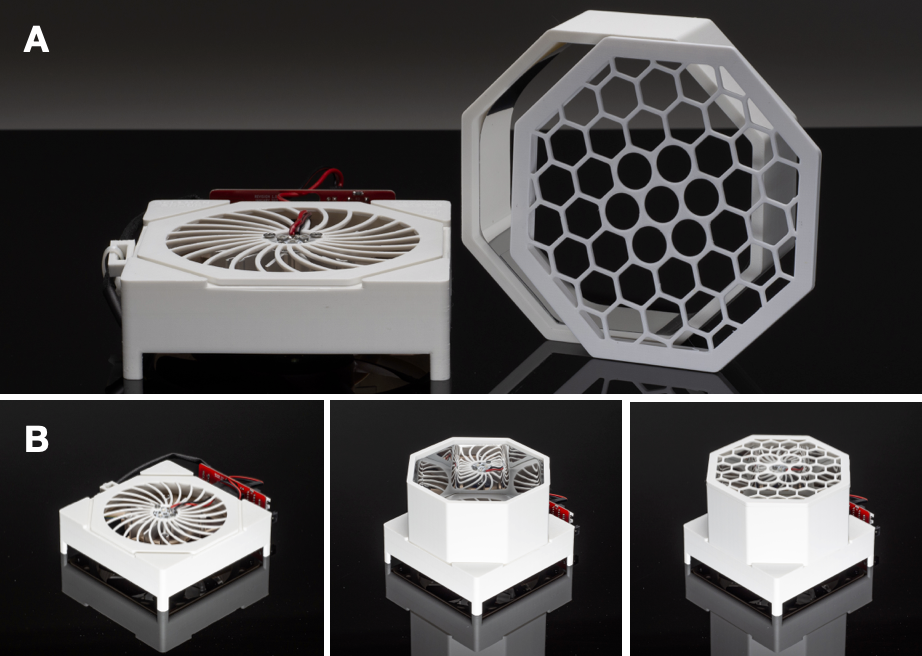
\includegraphics[width=\textwidth]{"./fig1.png"}
	\caption{(A) Unassembled WPP device comprised of a vessel holder, reaction chamber and standardized base fitted with a digital driver board. (B) Modular apparatus assembly.}
\end{figure}
A WPP device consists of a base, reaction module and reactor driver (Figure 1A).
The base houses the photon source and cooling fan.
The reaction module is comprised of a reflective reaction chamber and rigid vessel holder.
A digital driver board, analog driver board or simple circuit integrating a commercial light emitting diode (LED) driver can be fitted to the base to drive the reactor.

Each component is highly versatile, and apparatus assembly is fully modular (Figure 1B).
Through variation of each component, one can quickly produce bespoke WPP devices to meet specific research needs.

The WPP is a living project.
We encourage duplication, modification and expansion of our designs.
If you would like to contribute to the WPP project or notice a problem, please consider opening a pull request or issue on GitHub.

\section{Fabrication}

WPP devices are simple to fabricate.
To fabricate a WPP device, you'll need a soldering iron, electronics tweezers, thin nose pliers and a screwdriver at minimum.
The fabrication process is divided into three parts:

\begin{itemize}
	\item Base and photon source fabrication, described in \autoref{SEC:base}
	\item Reaction module fabrication, described in \autoref{SEC:enclosure}
	\item Reactor driver electronics fabrication, described in \autoref{SEC:electronics}
\end{itemize}

A WPP device is made up of many commercially available parts.
This guide assumes that you have already procured those parts.
The project repository provides README files containing a bill of materials for each component with part numbers and suggested vendors.

\subsection{Base and Photon Source} \label{SEC:base}

\begin{figure}[H]
	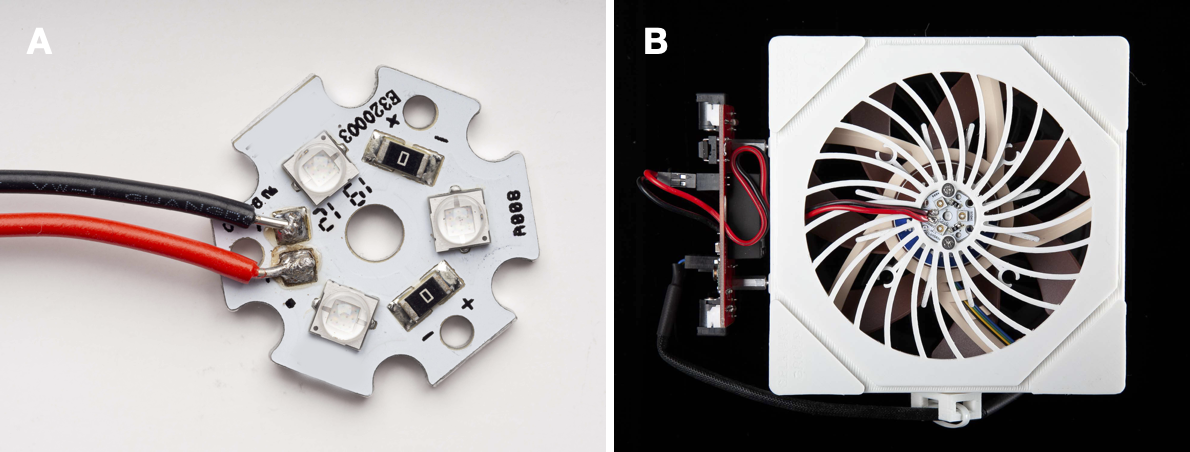
\includegraphics[width=\textwidth]{"./fig2.png"}
	\caption{(A) Commercial 20 mm LED star mounted with 450 nm Cree, Inc. XT-E LEDs. (B) Top-down view of WPP base depicting integrated LED star.}
\end{figure}

The WPP architecture uses industry standard 20 mm ``LED star'' circuit boards mounted with 3 high-intensity LEDs to deliver photons to reaction vessels (Figure 2A).
LED stars are commercially available or can be easily fabricated.
The range of wavelengths provided by a LED star depends upon the emission profile of the mounted LEDs.
\textbf{\textit{Through variation of the LED star integrated into a WPP base (Figure 2B), the user can control the wavelengths of light delivered by the photon source to a reaction vessel.}}
An aluminum heatsink and cooling fan are integrated to keep the LED star from overheating.

A list of LED stars tested with the WPP platform is available in the 'photon-source-leds' subdirectory of the project repository.
It is easiest to use LED stars with pre-mounted LEDs.
Otherwise, you can fabricate custom LED stars with discrete LEDs and bare LED star circuit boards.
Custom LED star production requires a reflow oven.
All LEDs must have a maximum drive current of 1000 mA or higher.

\begin{figure}[H]
	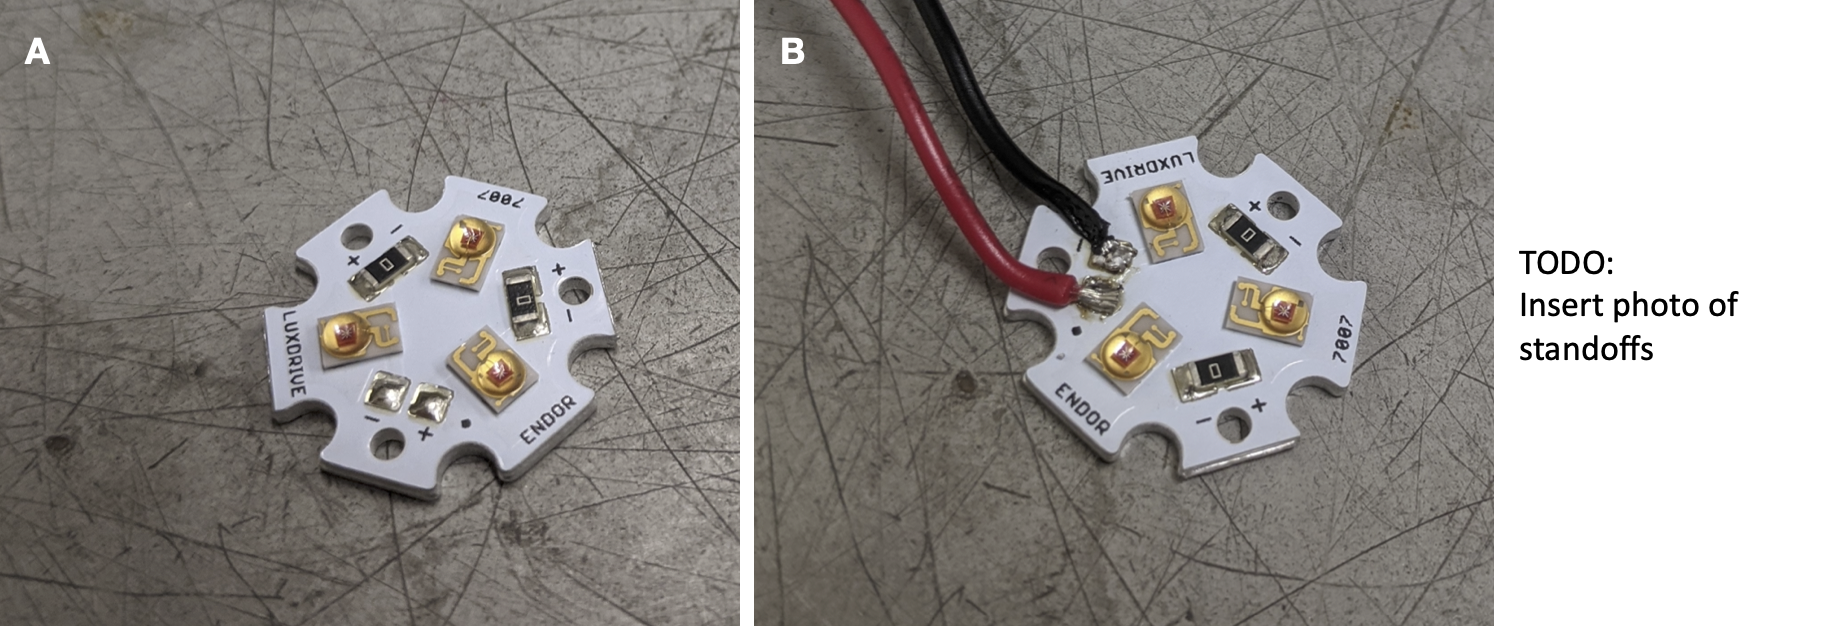
\includegraphics[width=\textwidth]{"./fig3.png"}
	\caption{(A) Unsoldered commercial LED star. (B) LED star with leads. (C) Connectors on other end of leads. (D) Connector sealed with heat-shrink tubing.}
\end{figure}

Fabrication of a WPP base begins with preparation of an LED star.
Solder leads onto your LED star, using the red positive and black negative convention (Figure 3A---B).
We recommend 22-gauge solid core wire.
This is often sold as "standard hookup" wire.
Soldering may be challenging, as the LED star itself will resist efforts to heat it.
Using lead-based solder with a low melting point may help.

Solder a connector to the end of the LED star.
Ensure the connection between the connector and wire is strong and has plenty of solder (Figure 3C).
Using heat-shrink tubing, seal the connection (Figure 3D).

\begin{figure}[H]
	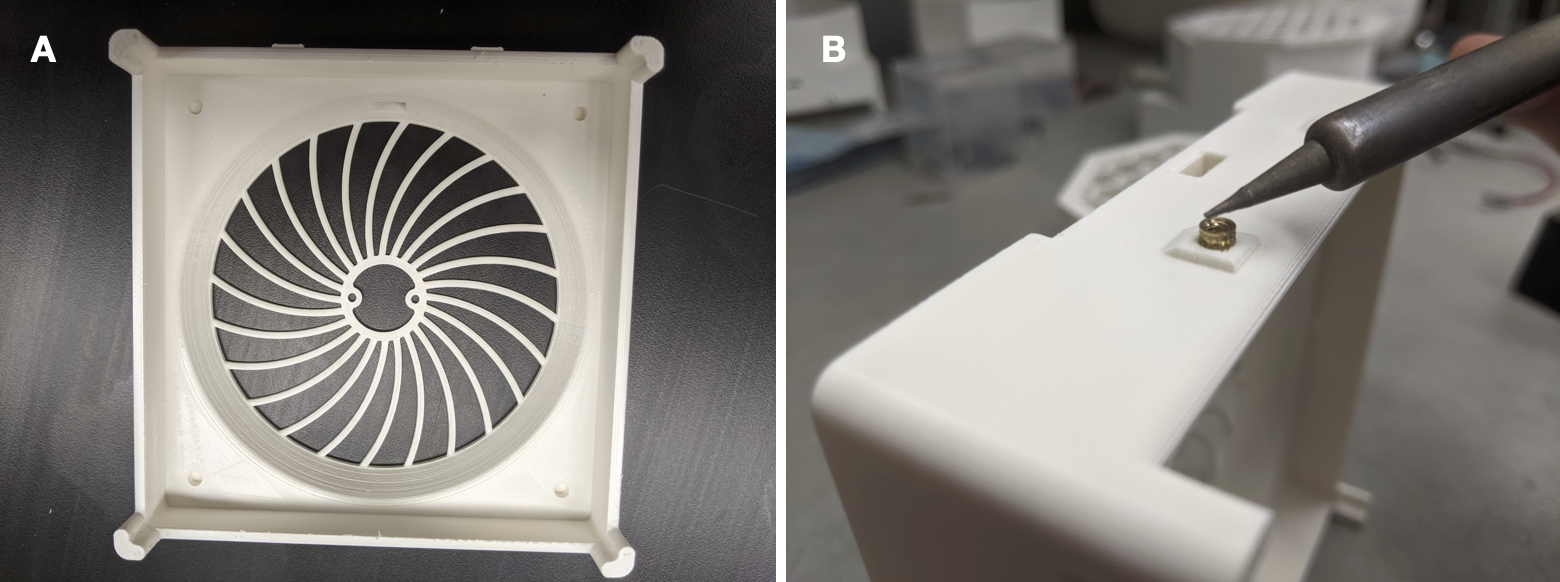
\includegraphics[width=\textwidth]{"./fig4.png"}
	\caption{(A) 3D-printed WPP base. (B) Securing a threaded inset into base.}
\end{figure}

Next, 3D-print a base enclosure and cable anchor.
Models for both are provided in the 'photoreactor-base' subdirectory of the project repository (Figure 4A).
The same base is shared by all WPP devices.

When interacting with the design files in our repository you will see several filetypes.
We have designed the WPP enclosure using Autodesk's Fusion 360 and included f3d design files for those who wish to extend or modify our designs.
Interacting with f3d files requires a Fusion 360 license, which is free for students and educators.
You will also find stl files in the repository.
These are common 3D-model exchange files that can be viewed with 3D modeling programs or printed with 3D-printers.

We recommend white PLA as the printing material. We have also used white ABS.
If you are printing yourself, follow the instructions provided by the manufacturer of your 3D-printer.
You will need to enable support material in your 3D slicer when printing the base enclosure.
We have successfully printed using the following printers:

\begin{itemize}
	\item Creality Ender 3
	\item Stratasys uPrint SE Plus
	\item Ultimaker 3 Extended
\end{itemize}

Any company or shop offering 3D printing as a service should accept our stl files without modification.
Once your base and cable anchor are printed, you may need to remove excess material with a razor blade or exacto-knife.

Each base contains seven threaded inserts.
These allow components such as an analog driver board and fan to rigidly attach to the base with screws.
Use a soldering iron to carefully heat the threaded inserts while pushing them into their cavities to set them (Figure 4B).

\begin{figure}[H]
	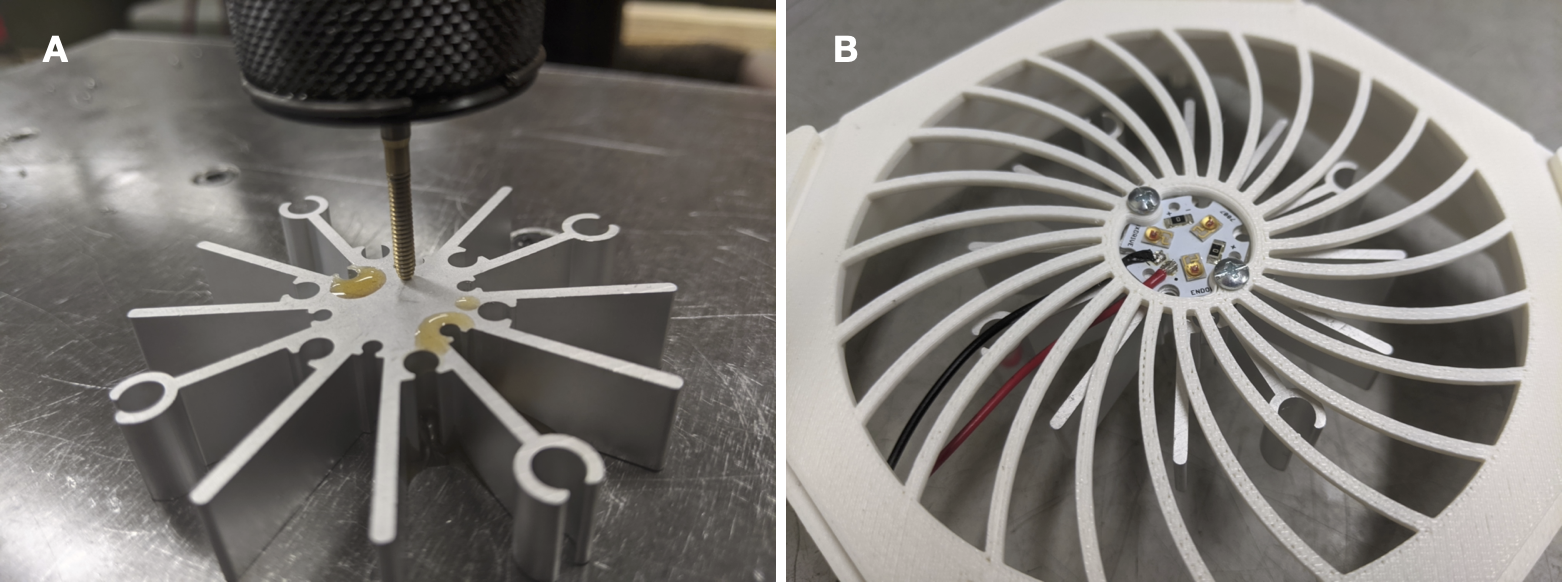
\includegraphics[width=\textwidth]{"./fig5.png"}
	\caption{(A) Tapping aluminum heatsink. (B) LED star and heatsink installed into WPP base.}
\end{figure}

Now tap an aluminum heatsink for imperial 4-40 machine screws.
We used thread-forming tap: OSG 1400105300 with a pneumatic ``air-tapper'' (Figure 5).
The heatsink can be tapped by hand.
You only need to tap two of the innermost holes.

Install the LED star and heatsink into the WPP base using 1/4'' screws.
Ensure the LED wires face towards the hole in the side of the printed base.

\begin{figure}[H]
	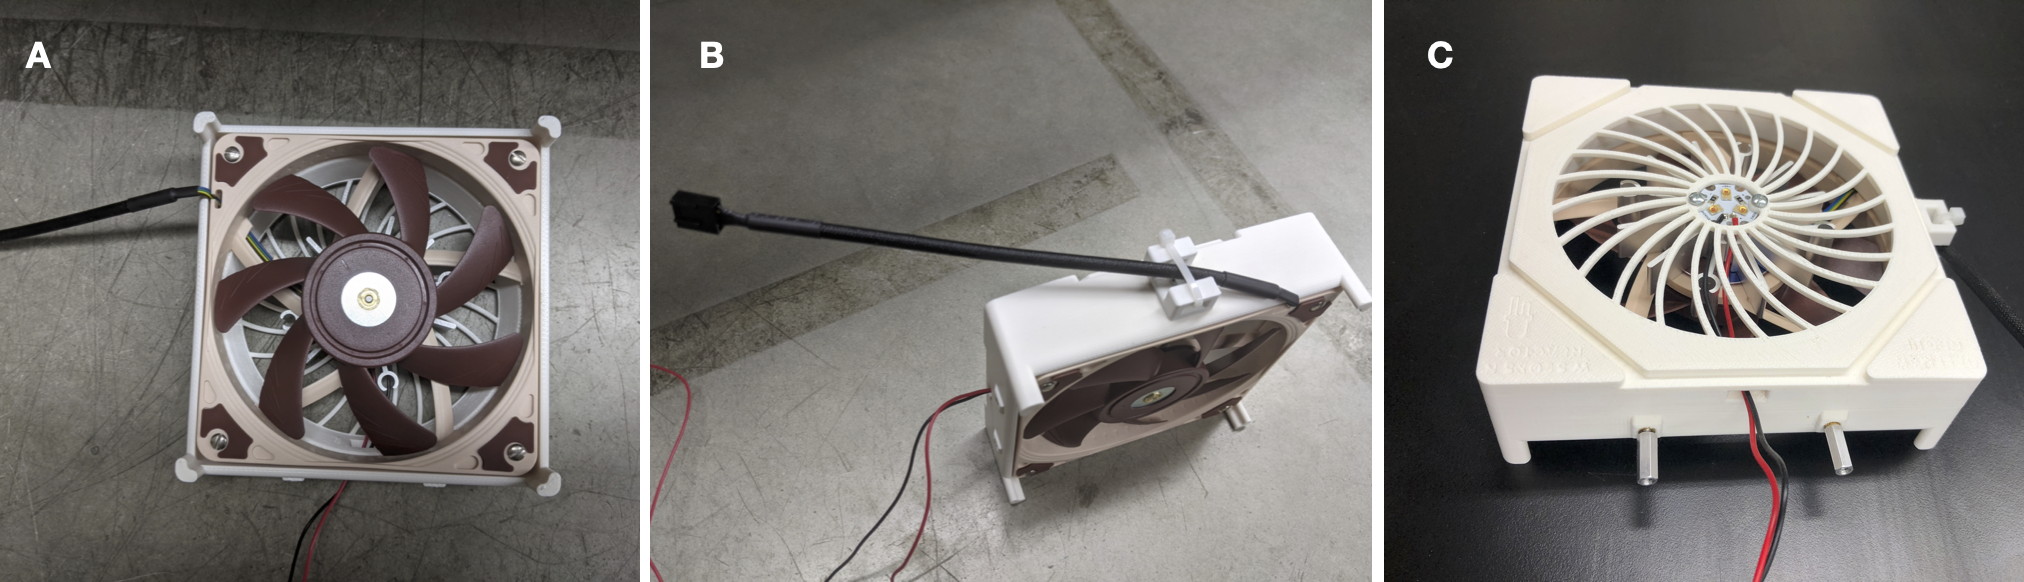
\includegraphics[width=\textwidth]{"./fig6.png"}
	\caption{(A) Integrated Fan. (B) Installed cable anchor with captured fan cord. (C) Metal standoffs screwed into base.}
\end{figure}

Install the fan.
Pay special attention to the orientation of the fan, including the location of the cord (Figure 6A).
Use 3/4'' screws here.
Then, install the cable anchor using a 1/4'' screw.
Use a zip tie to capture the fan cord (Figure 6B).
Finally, screw in the threaded standoffs (Figure 6C).
Your WPP base is now ready for use.

\begin{figure}[H]
	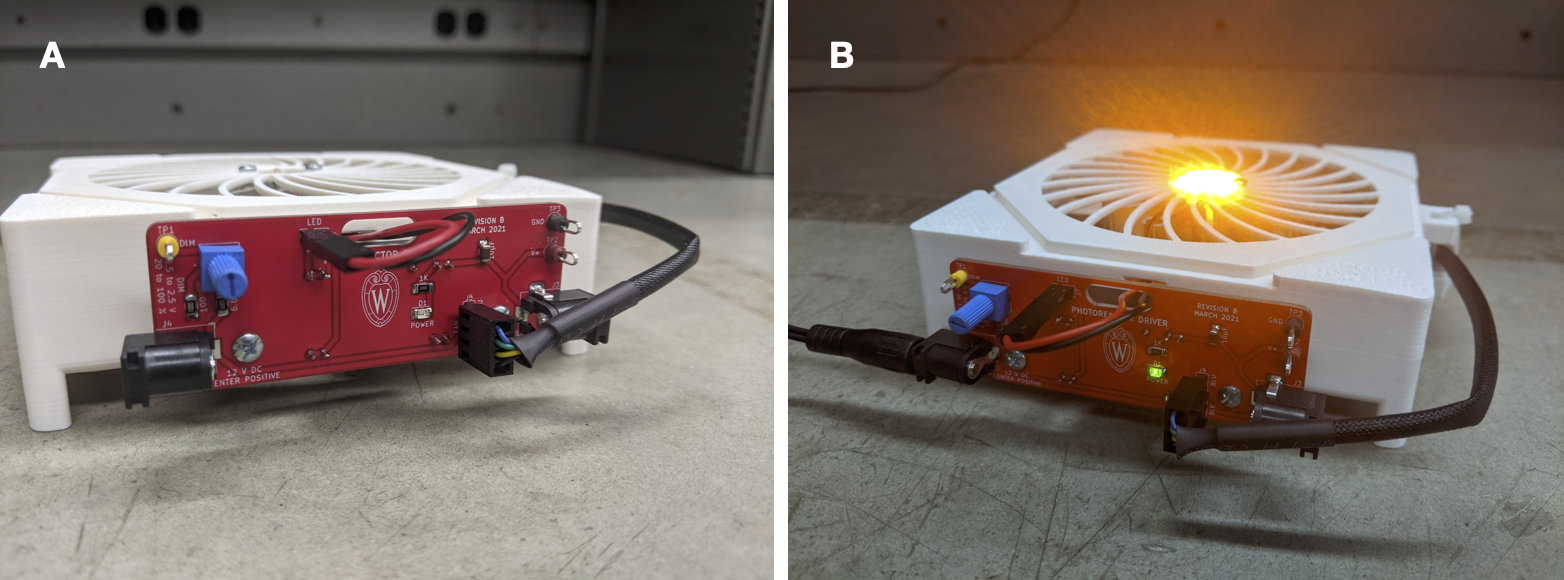
\includegraphics[width=\textwidth]{"./fig7.png"}
	\caption{A WPP base fitted with an analog driver board with and without power.}
\end{figure}

To test the photoreactor base, simply screw a driver board to the threaded standoffs and plug the LED and fan into the board.
Pay special attention to the orientation of both connectors.
Your base should light up upon connection to power (Figure 7).
Remember to use proper eye protection.

\clearpage

\subsection{Reaction Module} \label{SEC:enclosure}

\begin{figure}[H]
	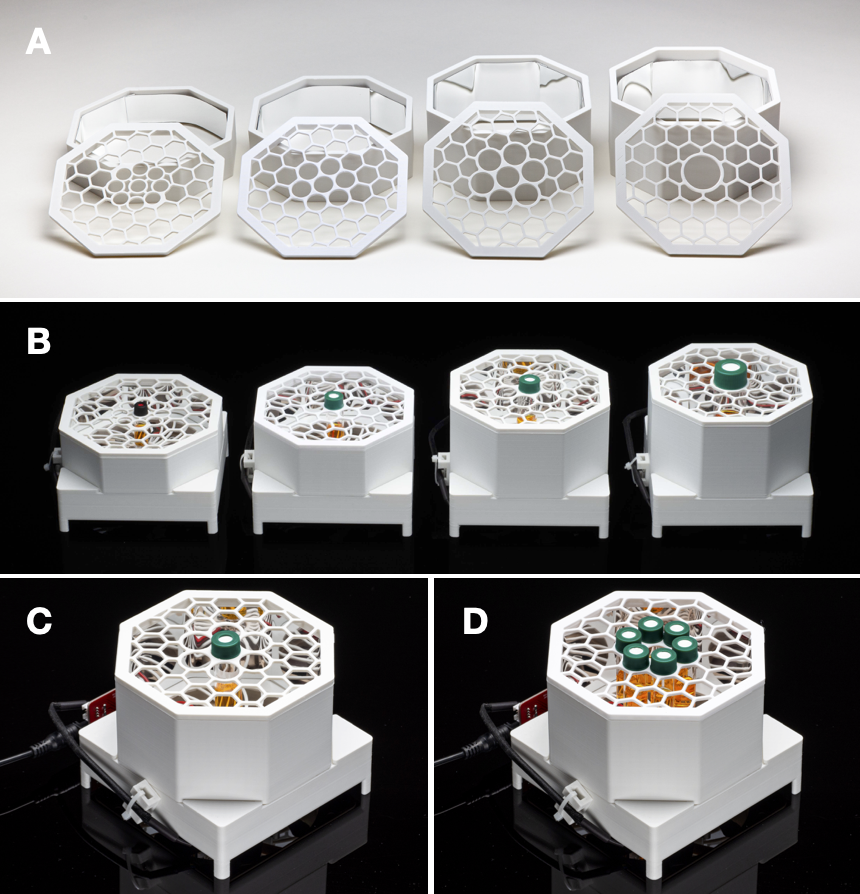
\includegraphics[width=\textwidth]{"./fig8.png"}
	\caption{(A) Provided reaction modules for 2-, 4-, 8- and 24-mL vials. (B) WPP devices fitted with the provided reaction modules. (C) Single and (D) multiple reaction configurations for provide 4-mL module.}
\end{figure}

A WPP reaction module consists of a reaction chamber and vessel holder.
By modifying chamber height and adjusting holder geometry, one can produce modules compatible with reaction vessels of various types and sizes.
Fusion360 designs and stl models for modules compatible with 2-, 4-, 8- and 24-mL vials are provided in the 'photoreactor-reaction-modules' subdirectory of the project repository (Figure 8A—B).
Template reaction chamber and vessel holder Fusion360 designs are provided in the same directory.

We encourage you to design your own reaction modules if those provided in the project repository do not meet your needs.
If you do, we suggest you add your designs to the WPP repository so that others may benefit from your efforts.

A single reaction module can offer multiple layouts for reaction vessel placement.
For the provided modules, two vessel placement configurations exist.
First, the single reaction configuration, where one vessel is placed in the center of the module directly above the photon source (Figure 8C).
This configuration exposes one vessel to maximum light intensity.
Second, the multiple reaction configuration, where multiple vessels are placed in a circle around the photon source (Figure 8D).
This configuration exposes each vessel to less light relative to the single reaction configuration but provides equivalent exposure to each vessel.
\textbf{\textit{Through variation of the reaction module, the user can configure the reaction vessel type, size and placement within a WPP apparatus.}}

To fabricate a reaction module, simply 3D-print a reaction chamber and vial holder of your own design or taken from the 'reaction-modules' subdirectory of the project repository.

\begin{figure}[H]
	\centering
	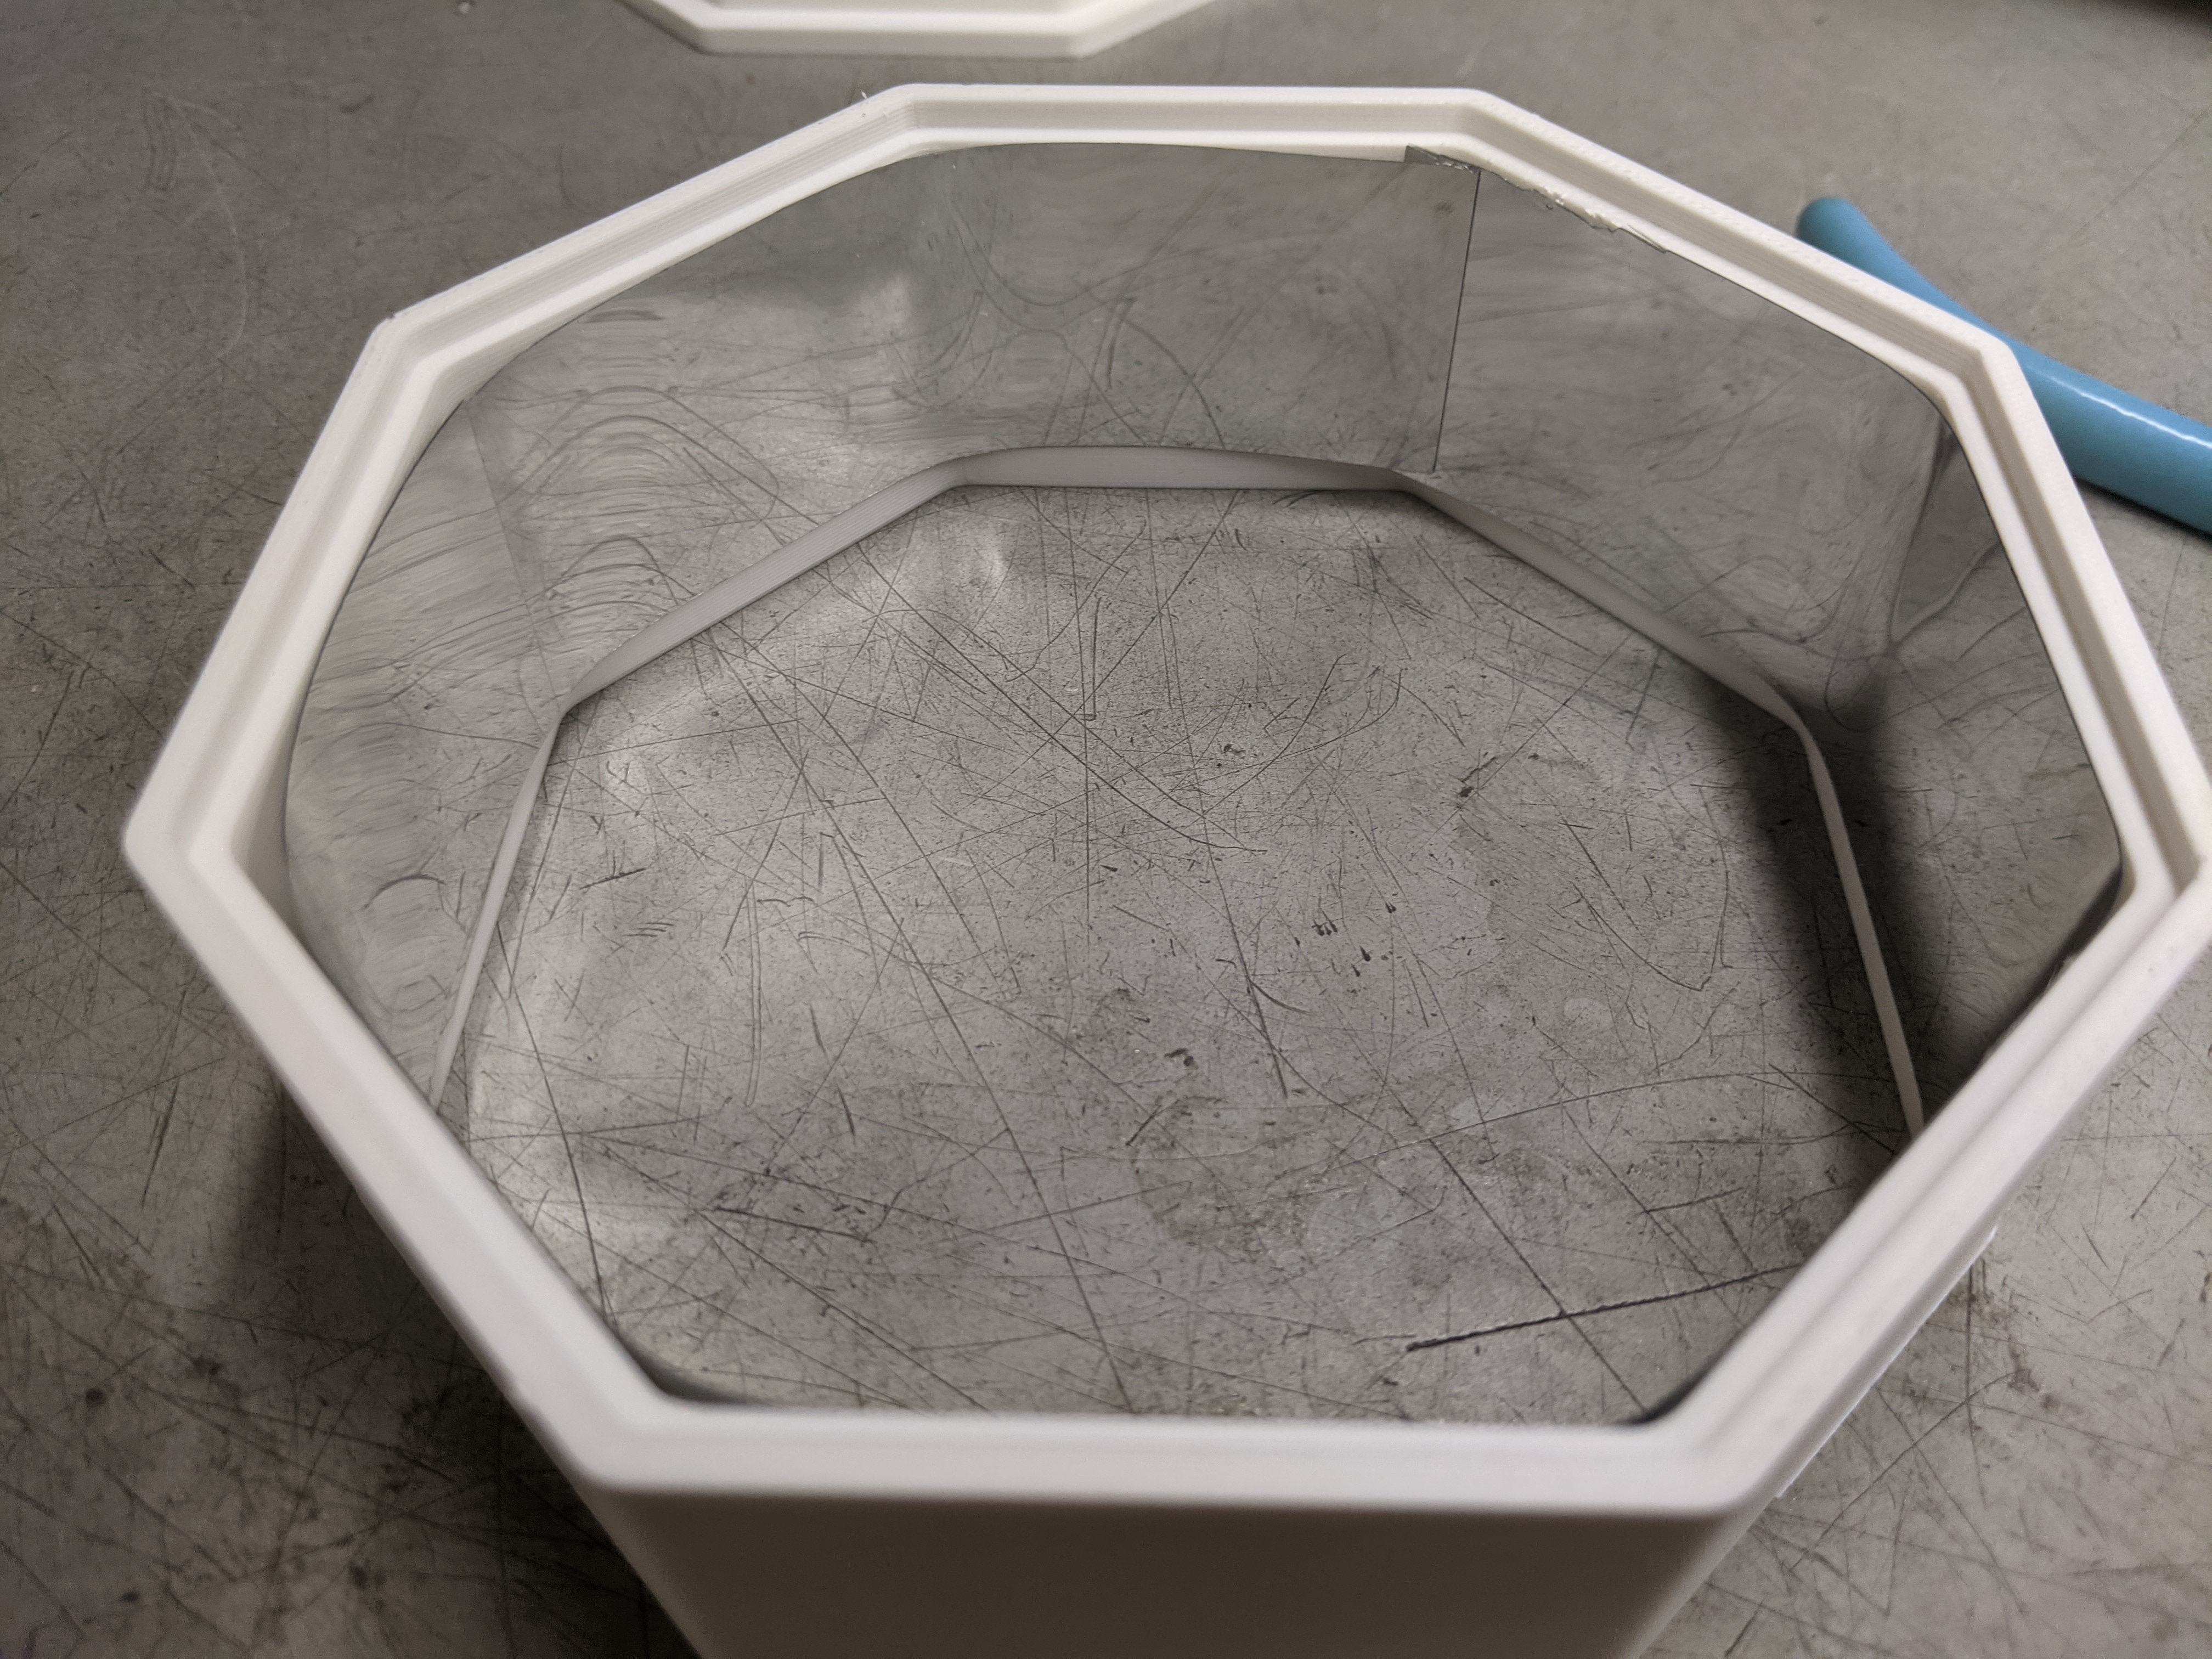
\includegraphics[width=\textwidth]{"./fig9.png"}
	\caption{(A) 4-mL reaction chamber. (B) Chamber lined with reflective material.}
\end{figure}

Once both parts are finished printing, cut reflective material to line the inside of the reaction chamber.
Remove the backing and stick the material to the chamber walls (Figure 9A---B).
It is fine to leave overlap around the interior.
The 3D printed vial holder requires no modification.
Your reaction module is now ready for use.

\clearpage

\subsection{Reactor Driver Electronics} \label{SEC:electronics}

\begin{figure}[H]
	\centering
	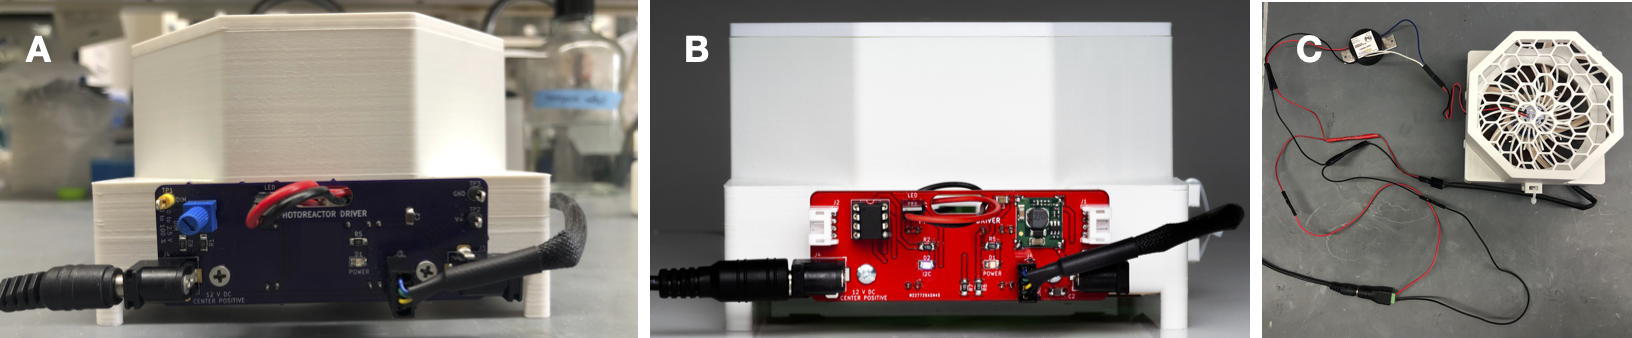
\includegraphics[width=\textwidth]{"./fig10.png"}
	\caption{(A) Analog driver board. (B) Digital driver board. (C) Simple driver circuit.}
\end{figure}

A WPP device can be driven using an analog driver circuit board, a digital driver circuit board or a simple electronic circuit with a commercial LED driver (Figure 10).
All provide power to the cooling fan and current to the LEDs.
All utilize 1000 mA LED drivers. 
\textbf{\textit{Each provides different configurational capabilities.}}

Both driver boards are built around Mean Well's LDD-1000L LED driver module.
This module delivers current up to one amp.
The current delivered can be controlled electronically in several different ways.
Users wishing to understand this design should refer to Mean Well's datasheet.
Refer to the "analog-driver-board" and "digital-driver-board" directories in the online repository for design files for each board.

The analog driver board is designed to be exceedingly simple to fabricate and use.
The circuit accepts DC 12 V through a barrel jack.
A small knob is used to adjust light intensity.
Fan speed is not adjustable.
\textbf{We recommend that chemists interested in adopting the WPP architecture first build and test the analog driver board.}
Refer to \autoref{SEC:analog-driver} for analog driver board fabrication instructions and further explanation.


The digital driver board is made to be incorporated into an I$^2$C-based digital control system.
In addition to power, these boards have 4-pin connectors to carry the I$^2$C serial data.
\textbf{We recommend that chemists experienced in electronics and interested in automation of WPP devices or taking advantage of I$^2$C peripherals to expand device functionality use the digital driver board.}
Refer to \autoref{SEC:digital-driver} for digital driver board fabrication instructions and further explanation.

The simple driver circuit allows for any commercial 1000 mA LED driver to be used with a WPP device.
Refer to \autoref{SEC:simple-driver} for further explanation.

When interacting with the design files in our online repository you will see several different filetypes.
These circuit boards were designed using KiCad, a free and open source electronics CAD software.
All KiCad files are contained within the ``kicad'' subdirectories.
You may modify and extend these designs however you like.

Those wishing to produce the analog driver board or digital driver board designs should refer to the 'gerber' subdirectory.
Within this subdirectory you will find zip files containing everything necessary for production of printed circuit boards (PCB) of each board design.
You may upload these zip files to PCB manufacturers when ordering copies of our designs.

\clearpage
\subsubsection{Analog Driver Board} \label{SEC:analog-driver}

\begin{figure}[H]
	\centering
	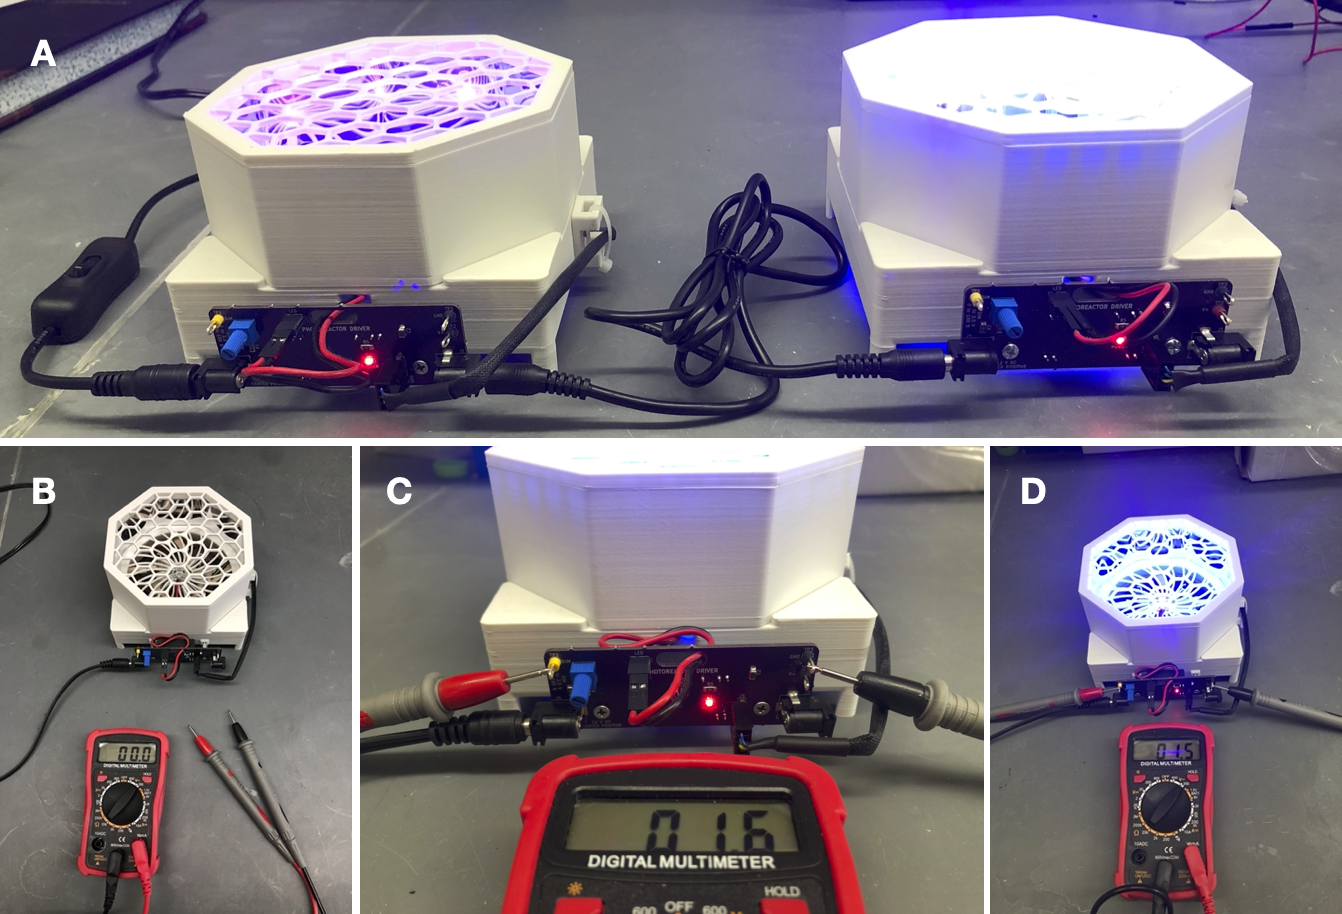
\includegraphics[width=\textwidth]{"./fig11.png"}
	\caption{(A) WPP devices fitted with analog driver boards connected in series. (B) Multimeter and WPP apparatus fitted with analog driver board. (C) Connection of multimeter to test points. (D) WPP apparatus at ~60 percent light intensity (1.5 V test point voltage)}
\end{figure}

\textbf{\textit{Through use of the analog driver board, one can reproducibly control WPP device light intensity via modulation of drive current.}}
This control is achieved through adjustment of the board-mounted potentiometer.
No firmware is required, and multiple WPP reactors can be connected in series to a single power source (Figure 11A).
However, fan speed isn’t adjustable and is maintained at maximum.
A full schematic of the analog circuit appears at the end of this section.
A bill of materials appears within the README file of the 'analog-driver-board' subdirectory of the project repository.

Relative light intensity can be determined using the analog driver board test points and a multimeter (Figure 11B-D).
The measured voltage can then be converted to relative light intensity using the values in Table 1.
These values are derived from Mean Well's datasheet for the analog board’s LDD-1000L LED driver and are not exact.

\begin{table}[H]
	\centering
	\begin{tabular}{cc}
		\centering
		\textbf{Test Point Voltage} & \textbf{Approximate Relative Light Intensity} \\
		2.5                         & 100\%                                         \\
		2.25                        & 90\%                                          \\
		2.00                        & 80\%                                          \\
		1.75                        & 70\%                                          \\
		1.5                         & 60\%                                          \\
		1.25                        & 50\%                                          \\
		1.00                        & 40\%                                          \\
		0.75                        & 30\%                                          \\
		0.5                         & 20\%                                          \\
		0.45                        & 0\%
	\end{tabular}
	\caption{Test point voltage to approximate relative LED intensity conversion.}
	\label{tab:analog-board-conversion}
\end{table}

To fabricate an analog driver board, first order analog driver PCBs from a PCB manufacturer. Your PCB manufacturer will send you bare boards of the type seen in Figure 12A.

\begin{figure}[H]
	\centering
	\includegraphics[width=\textwidth]{"./fig12.png"}
	\caption{(A) Blank analog driver board. (B) Analog driver board with labeled surface mount components.}
\end{figure}

Begin by soldering the surface mount components.
Refer to the analog driver schematic for part identities.
We recommend using thin solder, e.g. 0.015''.
The surface mount resistors and capacitors have no polarity.
The power indicator LED has a polarity---ensure that the small green line points towards ground (left).
Once finished, your analog board should look like that depicted in Figure 12B.

\begin{figure}[H]
	\centering
	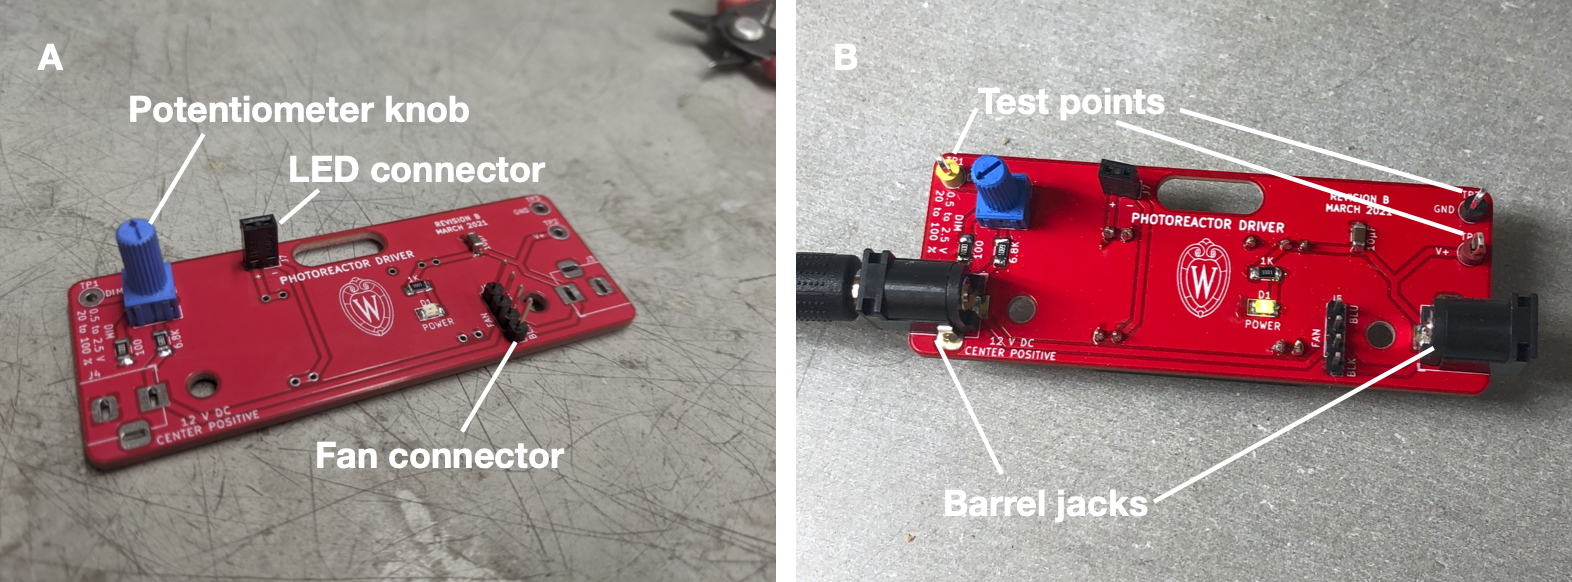
\includegraphics[width=\textwidth]{"./fig13.png"}
	\caption{(A) Analog driver board with potentiometer and connectors (B) Powered analog driver board.}
\end{figure}

Next, solder the connectors and potentiometer knob to the board (Figure 13A).
From now on we recommend standard gauge solder, e.g. 0.031''.
Then add the barrel jacks and test points.
With these added you may plug your board into power for the first time.
Either barrel jack can be plugged into power.
Your power indicator LED should illuminate (Figure 13B)

\begin{figure}[H]
	\centering
	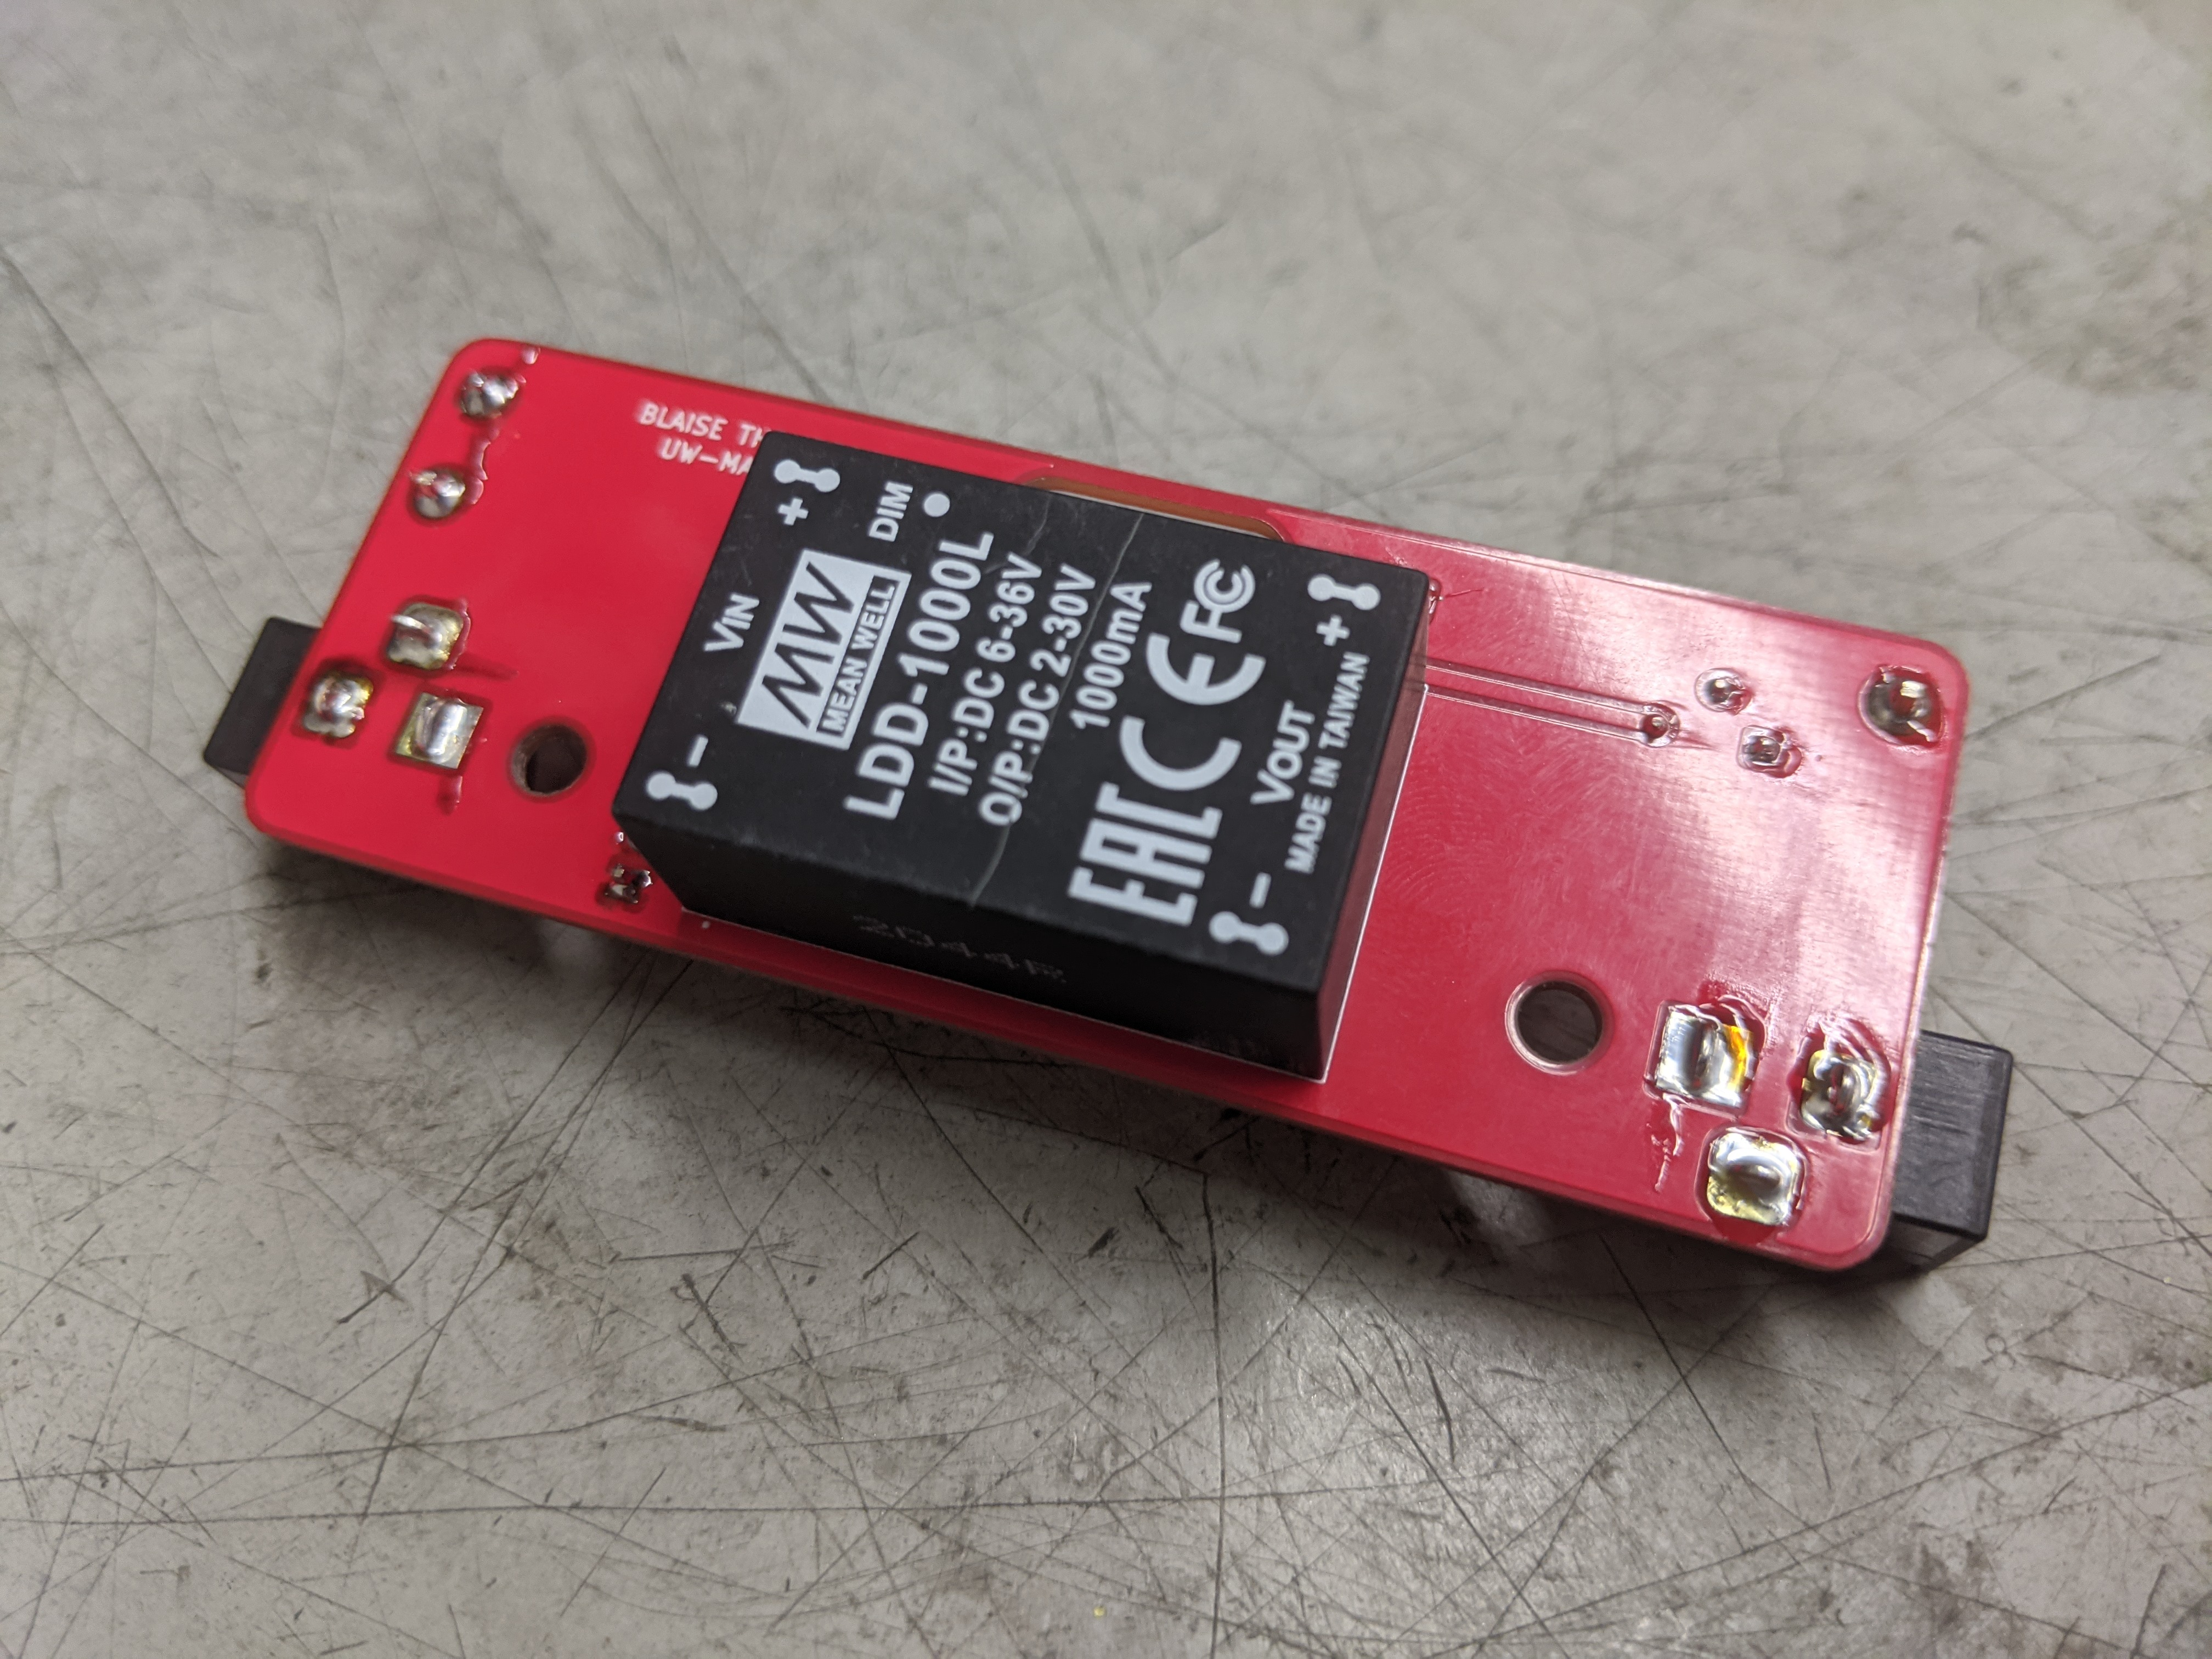
\includegraphics[width=\textwidth/2]{"./fig14.jpg"}
	\caption{Analog driver board fitted with Mean Well LDD-1000L LED driver.}
\end{figure}

Finally, solder the Mean Well LDD-1000L LED driver to the board (Figure 14).
This component goes on the back of the analog driver board.
The analog driver board is now ready for use.

\includepdf[landscape=true]{"../analog-driver-board/driver.pdf"}

\subsubsection{Digital Driver Board} \label{SEC:digital-driver}

\begin{figure}[H]
  \centering
  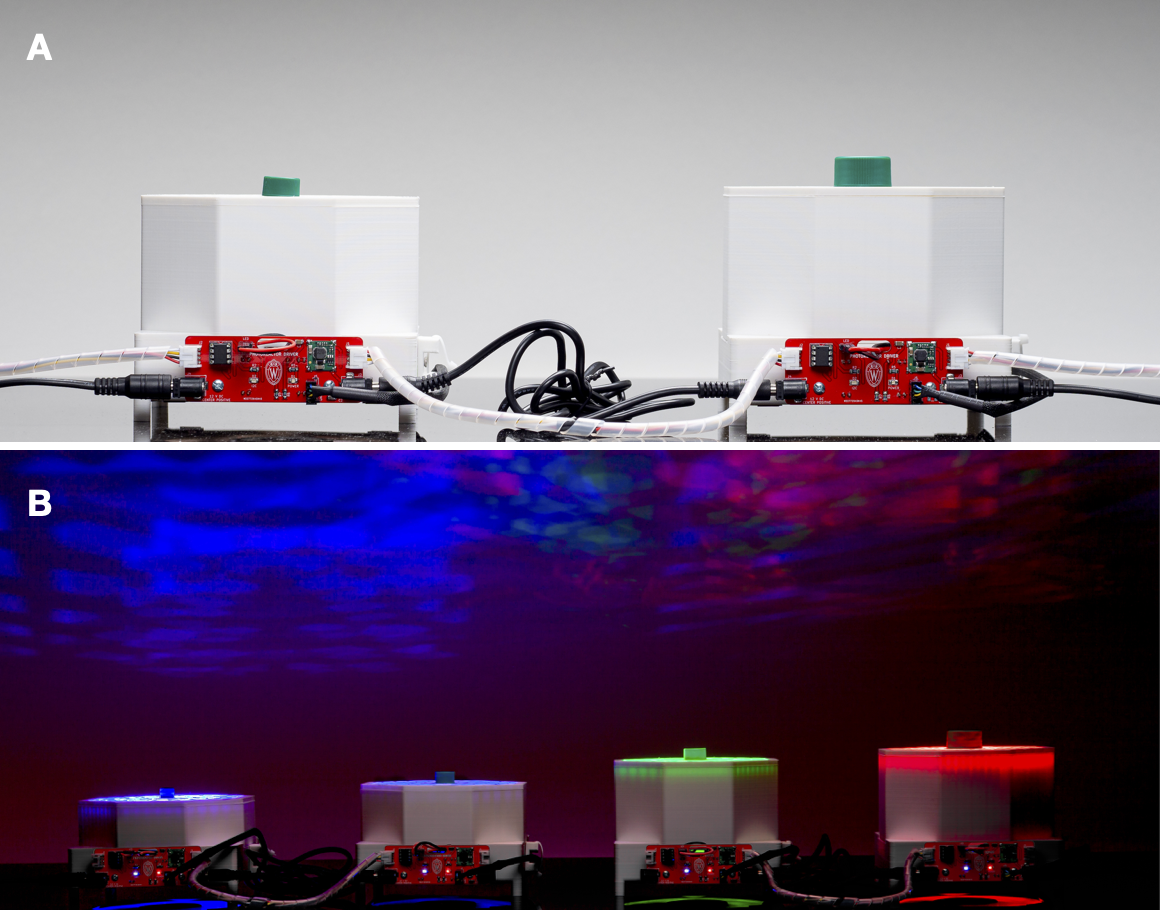
\includegraphics[width=\textwidth]{"./fig15.png"}
  \caption{(A) WPP devices fitted with digital driver boards connected in series. (B) Powered WPP devices connected in series.}
  \label{FIG:digital-driver-network}
\end{figure}

\textbf{\textit{Through use of the digital driver board, one can control WPP device light intensity and fan speed using pulse width modulation.}} This control is achieved by interfacing a control unit, like an Arduino Uno, to the digital driver board using custom firmware. Multiple WPP devices with digital driver boards can be connected to a single control unit and power supply (Figure 15). Open-source firmware for interfacing digital driver boards with an Arduino Uno control unit is provided in the project repository. Other peripherals can be connected to digital driver boards to expand functionality, but firmware must be produced to interface with them.

To fabricate a digital driver board, first order digital driver PCBs from a PCB manufacturer. You will be sent bare boards of the type seen in Figure 16A.

\begin{figure}[H]
	\centering
	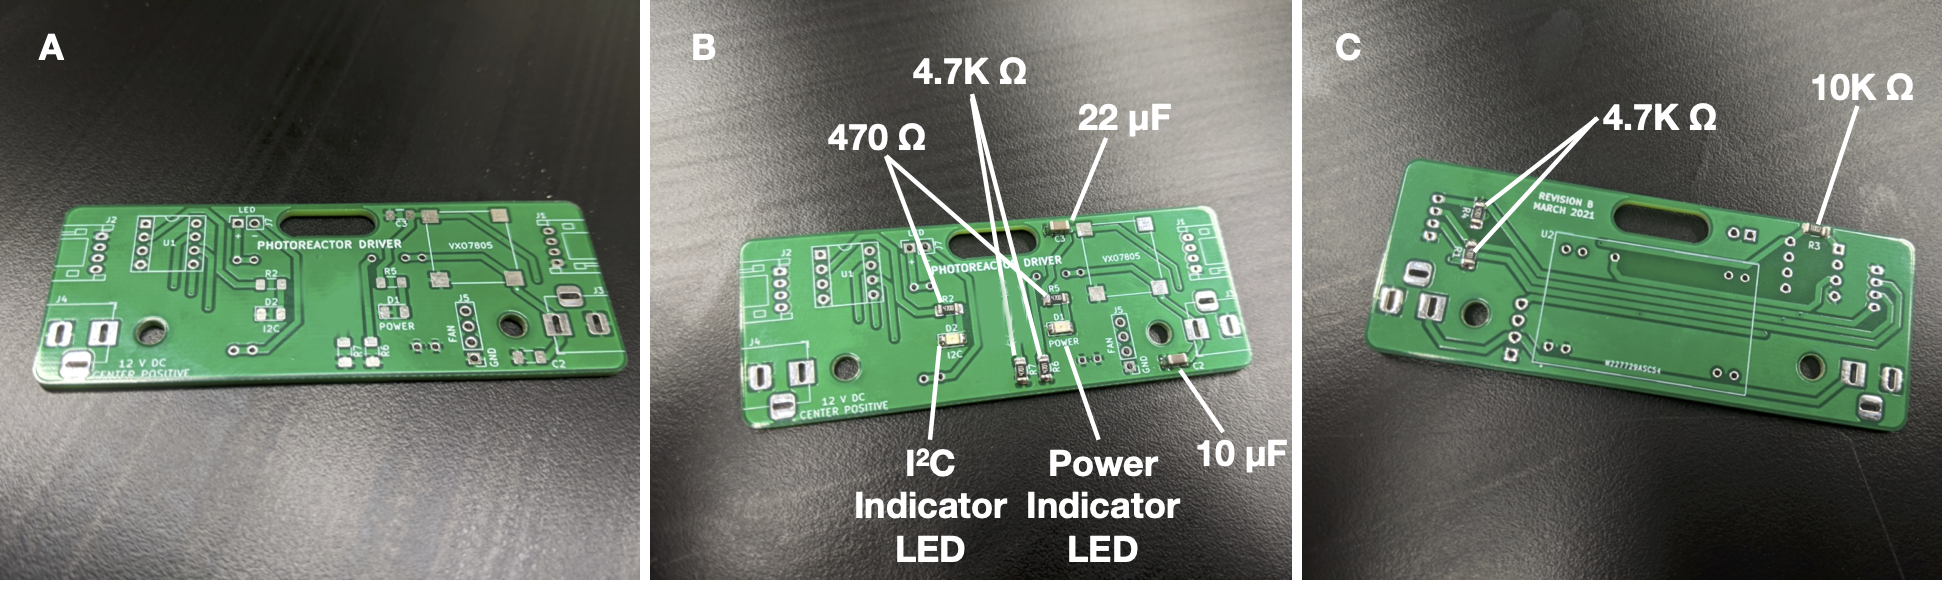
\includegraphics[width=\textwidth]{"./fig16.png"}
	\caption{(A) Blank digital driver board. (B) Front and (C) back of digital driver board with labeled surface mount components.}
\end{figure}

Begin by adding the surface mount components to the front and back of the digital driver board PCB.
Refer to the digital driver schematic for part identities.
We recommend using thin solder, e.g. 0.015''.
The surface mount resistors and capacitors have no polarity.
Both indicator LEDs have a polarity---ensure that the small green line on both points towards ground (left).
Once finished, your digital driver board should look like that in Figure 16B and C.

\begin{figure}[H]
	\centering
	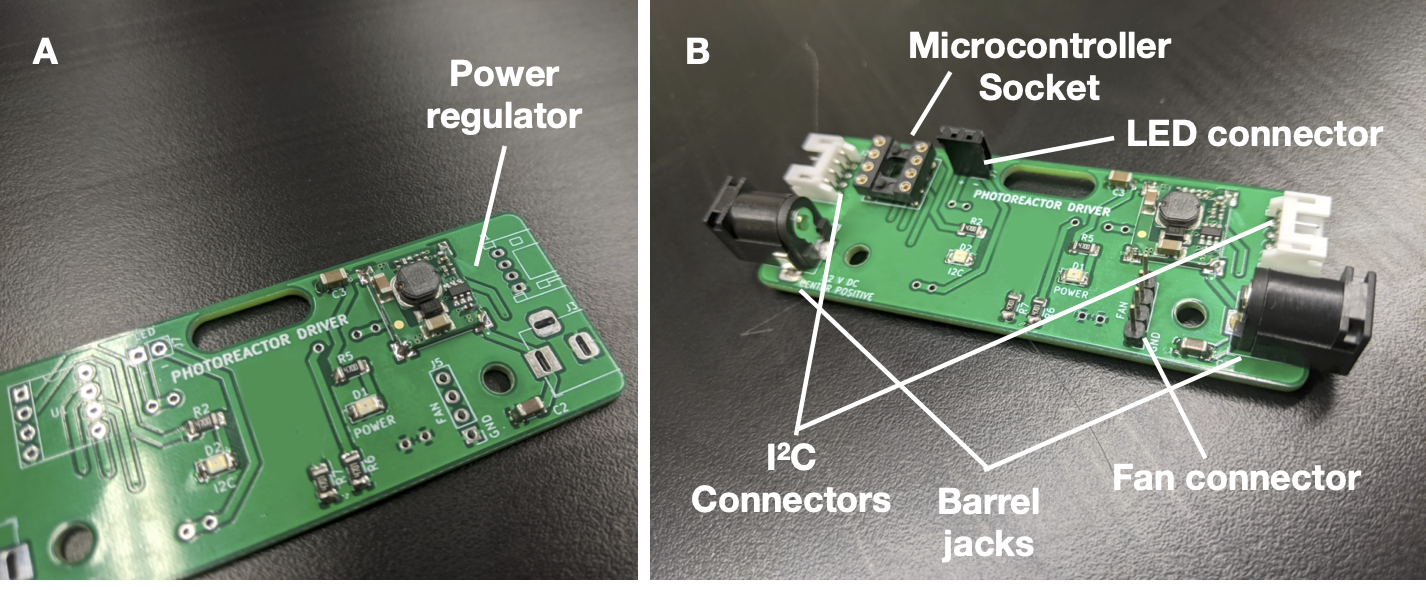
\includegraphics[width=\textwidth]{"./fig17.png"}
	\caption{(A) Digital driver board mounted with power regulator. (B) Digital driver board with connectors, microcontroller socket, JST connectors and barrel jacks.}
\end{figure}

Next, solder the power regulator to the board (Figure 17A).
Pay special attention to the orientation of the regulator.
From now on we recommend standard gauge solder, e.g. 0.031''.
Solder on the connectors, microcontroller socket, JST connectors and barrel jacks (figure 17B).

\begin{figure}[H]
	\centering
	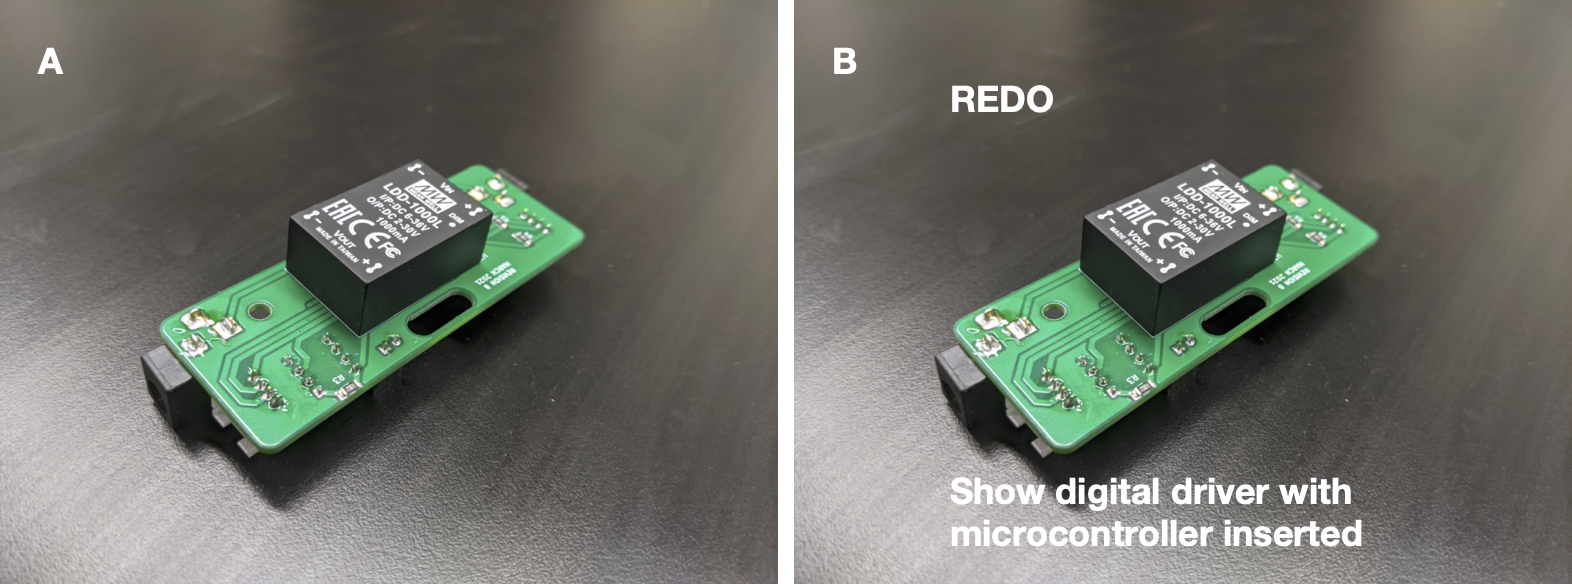
\includegraphics[width=\textwidth/2]{"./fig18.png"}
	\caption{Digital driver board fitted with Mean Well LDD-1000L LED driver.}
\end{figure}

Finally, solder a Mean Well LDD-1000L LED driver to the board (Figure 18).
This component goes on the back of the digital driver board.
Physical fabrication of the digital driver board is now complete.
However, a microcontroller programmed with the necessary firmware must be installed onto the board to make it functional.

Each digital driver board requires an ATtiny85 microcontroller to act as the ``brains'' of the board.
This microcontroller allows the digital driver board to serve as a peripheral in an I$^2$C network supervised by a central control unit.
I$^2$C is a standard protocol for communication between digital circuits.
To "communicate" with the control unit, the ATtiny85 microcontroller must be programmed with firmware.
Firmware for the ATtiny85 microcontroller is provided within the '/digital-driver-board/firmware' subdirectory of the project repository.
This firmware can be edited if needed or you can create your own. 

\begin{figure}[H]
	\centering
	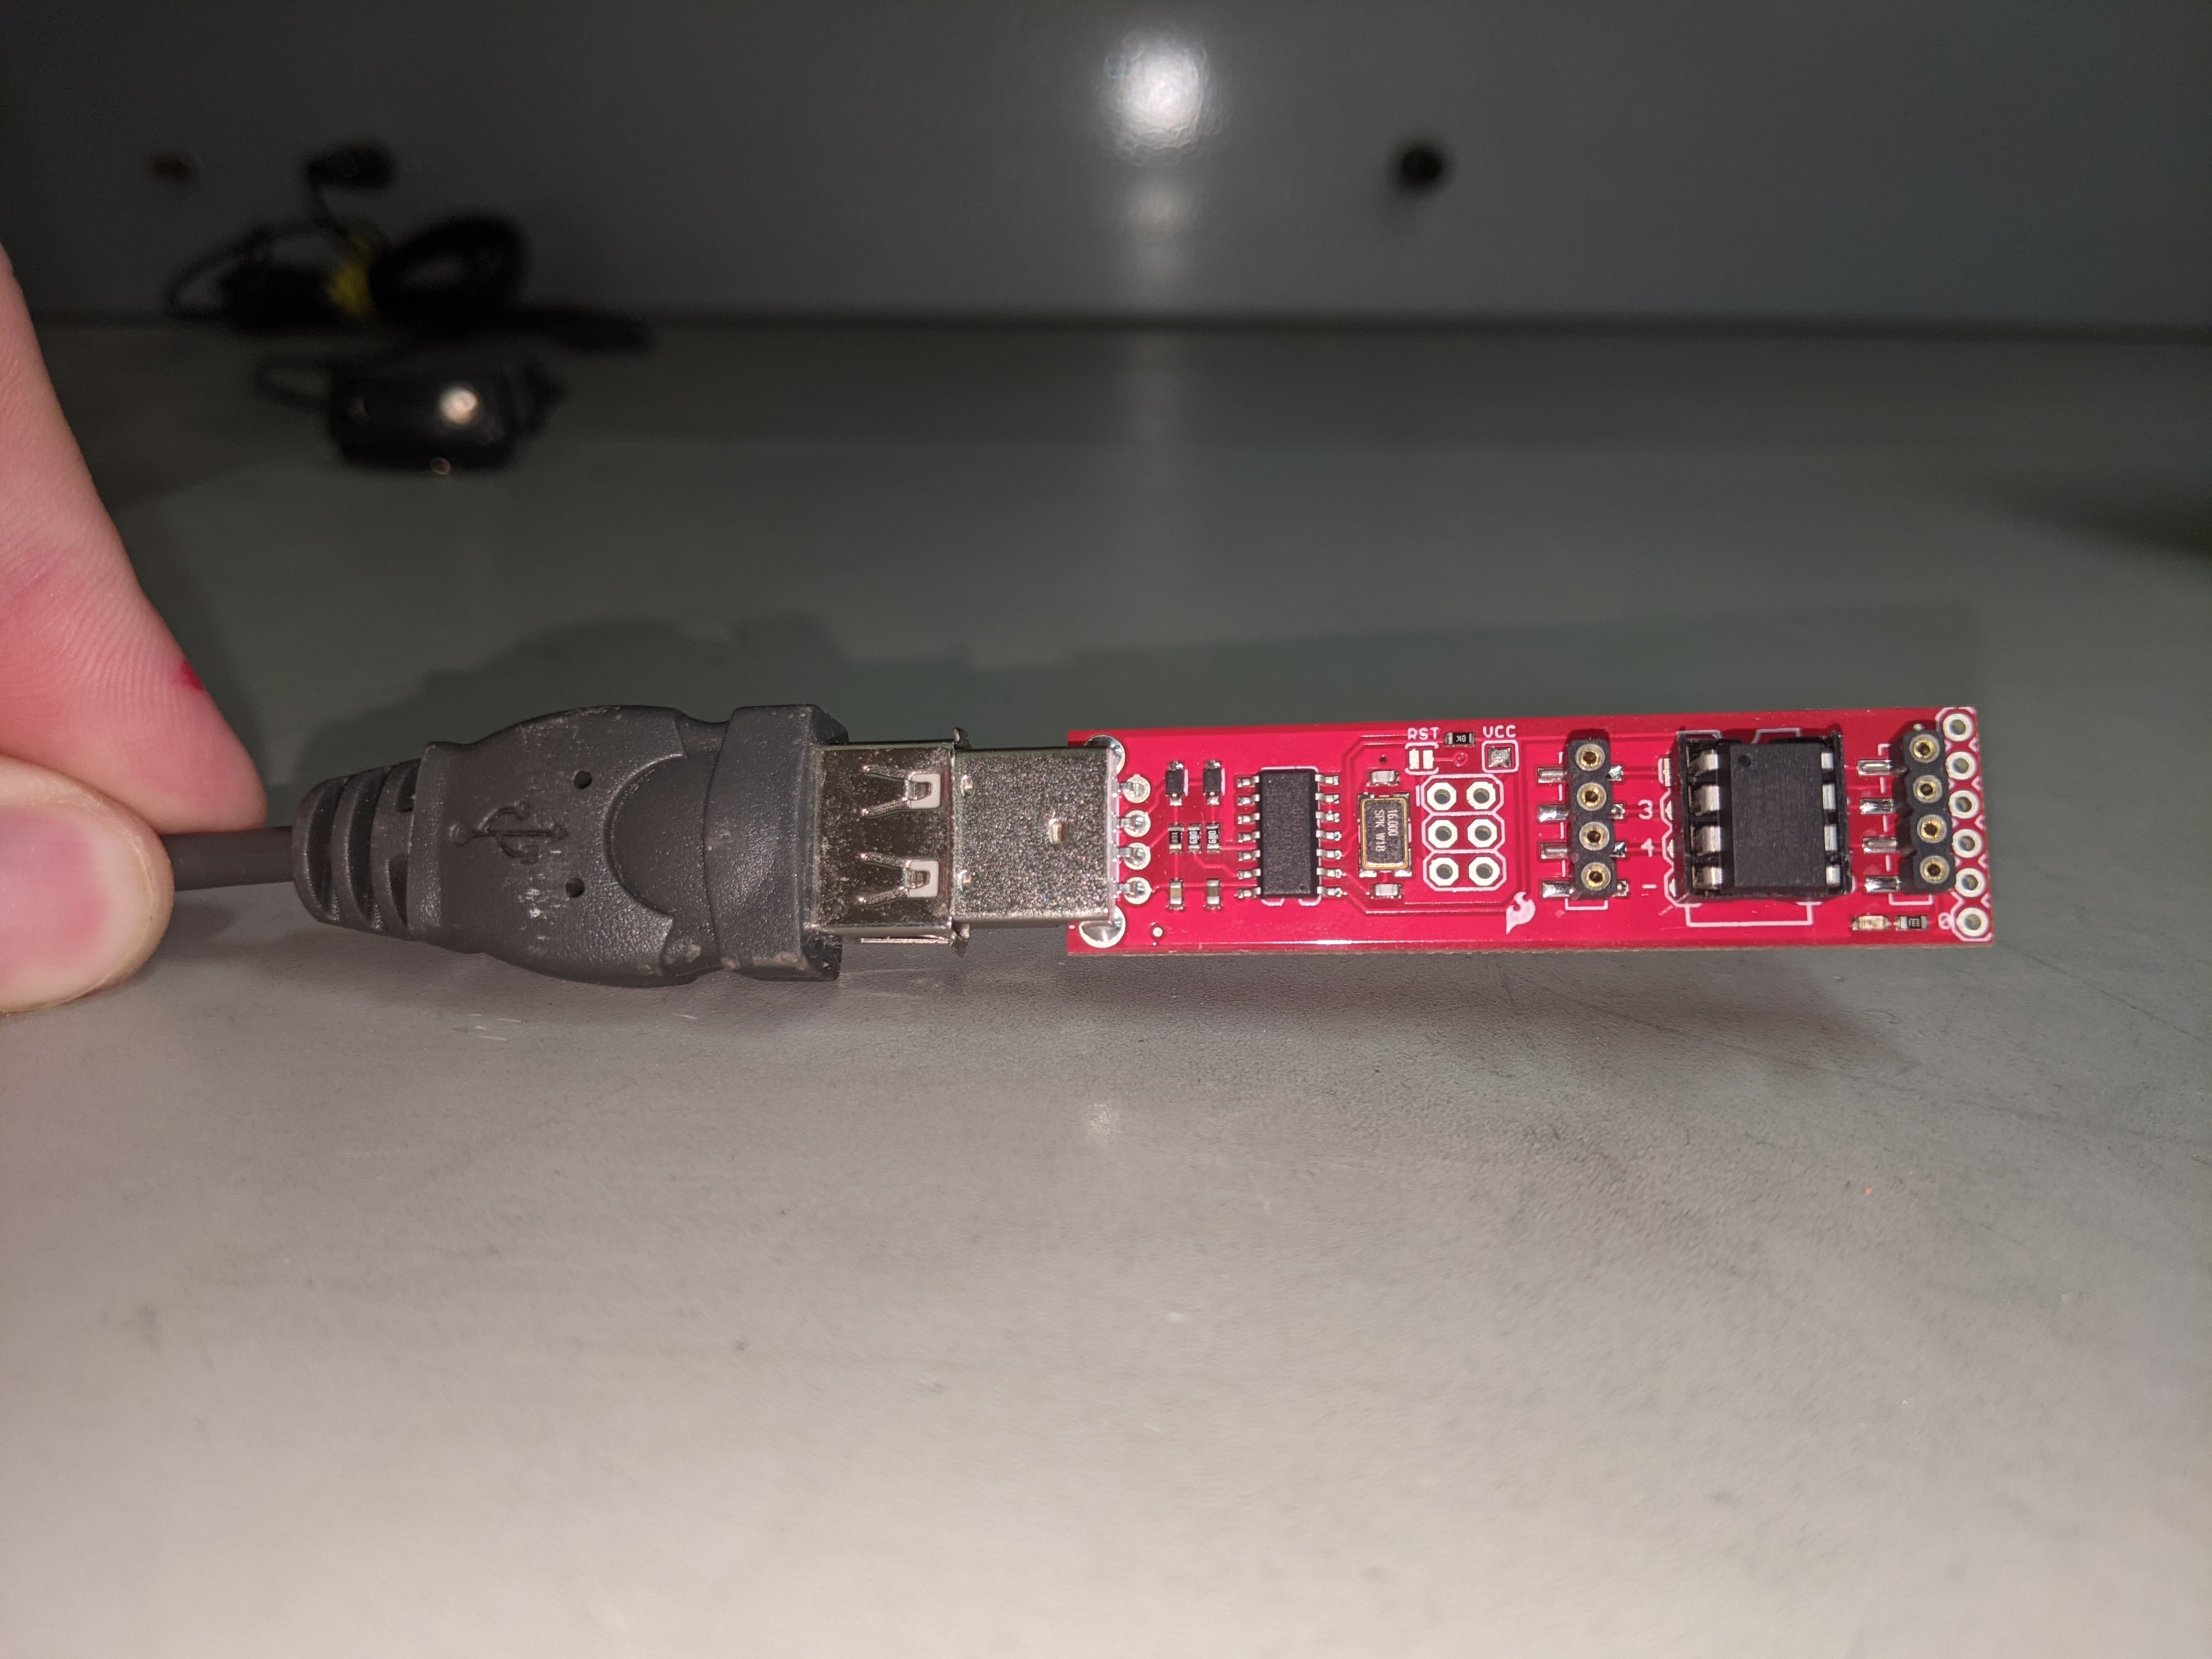
\includegraphics[width=\textwidth/2]{"./tiny-programmer.jpg"}
	\caption{An ATtiny85 microcontroller programmer purchased from SparkFun (item number PGM-11801).}
\end{figure}

\clearpage

We recommend using the Arduino IDE and a commercial programmer to program ATtiny85 microcontrollers (Figure 19).
Follow the instructions provided by the manufacturer of your programmer to program microcontrollers with the provided firmware.
Note that each digital driver board has an address that is defined at the top of the firmware file programmed onto each microcontroller.
You should change the address of each microcontroller to be unique within the ``network'' of all I$^2$C peripherals connected to a single control unit.
Multiple digital driver boards with unique addresses may be networked together onto one I$^2$C bus by simply daisy-chaining the boards together, as shown in \autoref{FIG:digital-driver-network}.
You should physically label each microcontroller you program with its address.

\begin{figure}[H]
	\centering
	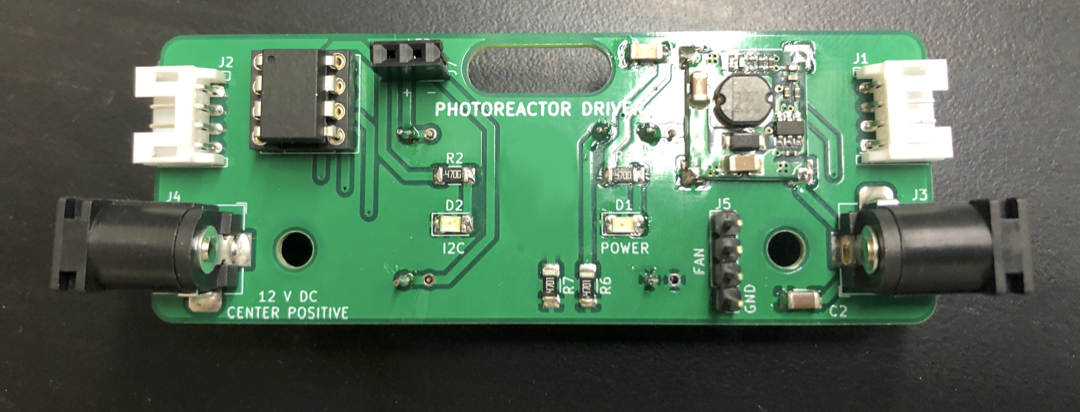
\includegraphics[width=\textwidth/2]{"./fig20.png"}
	\caption{Digital driver board with a ATtiny85 microcontroller installed.}
\end{figure}

Once you have a programmed ATtiny85 microcontroller, install it into the socket of the digital driver board as shown in Figure 21.
Ensure the notch in the microcontroller is facing the correct direction (up and to the left).
Your digital driver board is now ready for use with a control unit.

\begin{figure}[H]
	\centering
	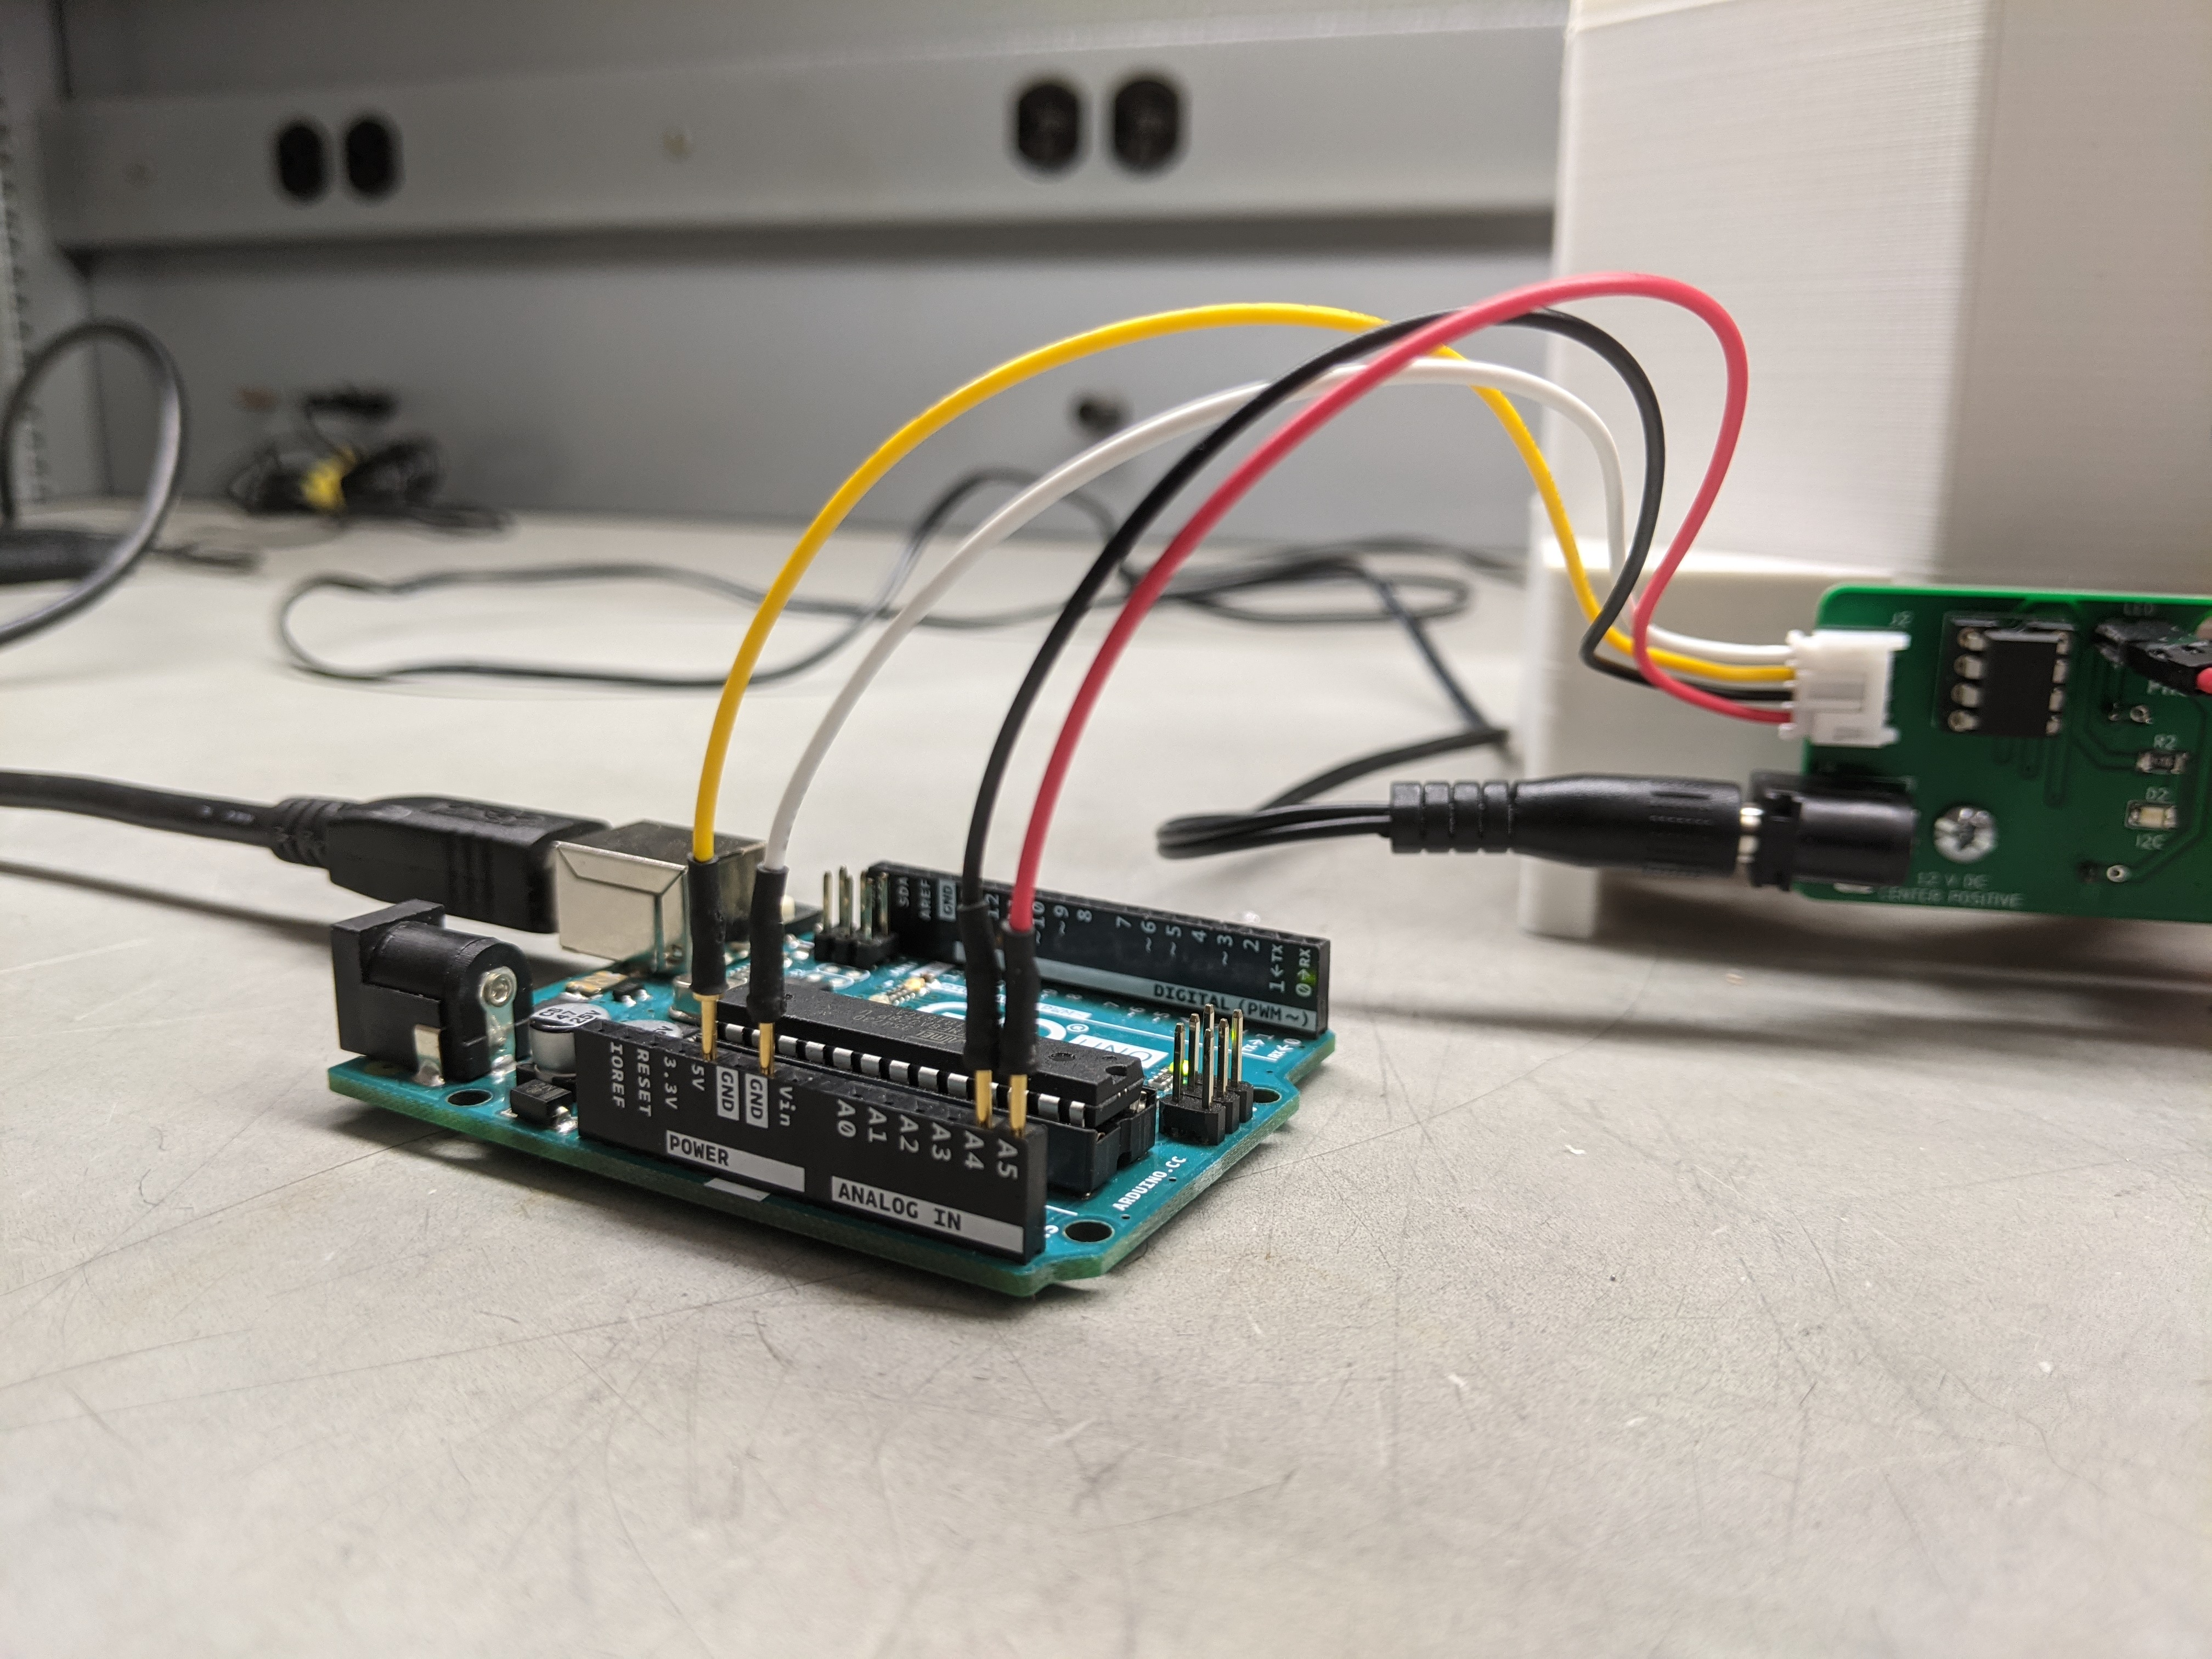
\includegraphics[width=\textwidth/2]{"./arduino-interface.jpg"}
	\caption{Digital driver board connected to an Arduino Uno.}
\end{figure}

\clearpage

There are many strategies one can employ to control digital driver boards.
We have provided firmware appropriate for using an Arduino Uno to control digital driver boards over a USB cable from any computer.
Find the firmware within the '/digital-controller/arduino-uno-controller/firmware' subdirectory of the project repository.
Flash this firmware onto an Arduino and connect at least the SCL, SDA, and GND pins to an Arduino Uno as shown in Figure 21.
This example firmware allows you to control multiple reactors by sending serial-over-USB commands from your computer.
Read the description at the top of the firmware file for details.

Many I$^2$C-compatible peripherals offering diverse functionalities are commercially available.
While the physical connectors may be different, our digital circuit is compatible with the following systems.

\begin{itemize}
  \item \href{https://learn.adafruit.com/introducing-adafruit-stemma-qt}{Adafruit STEMMA}
  \item \href{https://www.sparkfun.com/qwiic}{Sparkfun Qwiic}
  \item \href{https://www.seeedstudio.com/category/Grove-c-1003.html}{Seeed Grove}
  \item \href{https://store.ncd.io/?fwp_product_type=i2c-mini-modules}{NCD I2C Mini Modules}
\end{itemize}

I$^2$C peripherals in these families can be connected to digital driver boards to expand functionality, but software must be produced to interface with them.

\clearpage

\includepdf[landscape=true]{"../digital-driver-board/driver.pdf"}

\subsubsection{Simple Driver Circuit} \label{SEC:simple-driver}

\begin{figure}[H]
	\centering
	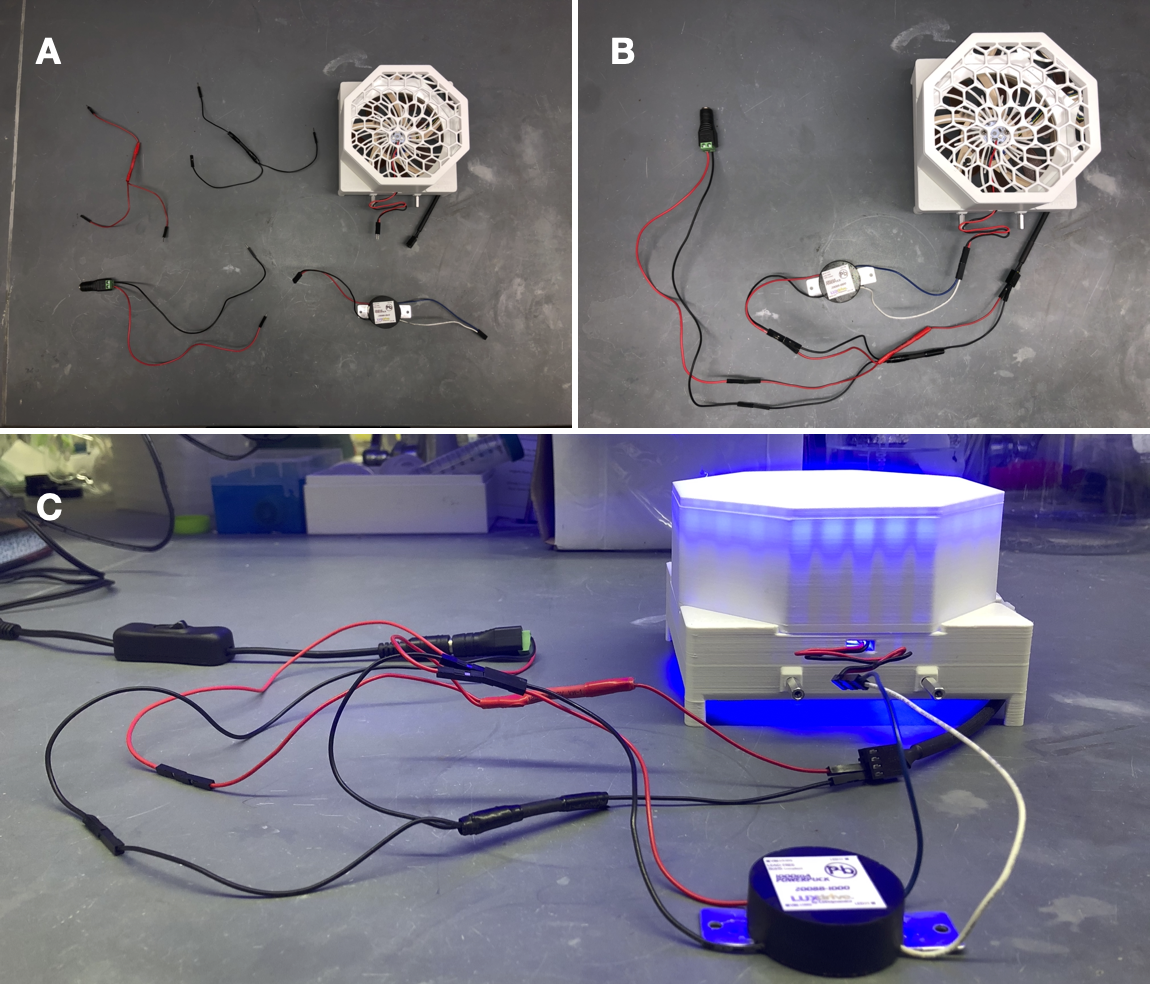
\includegraphics[width=\textwidth]{"./fign7.png"}
	\caption{(A) Unassembled pieces of the simple LED driver circuit integrating a LUXdrive 1000mA PowerPuck LED driver (Part number: 2008B-1000). (B) Assembled circuit. (C) Powered circuit.}
\end{figure}

The LED driver circuit shown in Figure 22 is the simplest way to drive a WPP apparatus.
Neither light intensity nor fan speed can be configured when using the simple LED driver circuit.
Both are maintained at maximum power.
However, no circuit board fabrication is required, and any commercial 1000 mA LED driver can be used.

\section{Operation}

Once a WPP apparatus is configured with the desired photon source, reaction module and reactor driver, it is ready to drive photoreactions.

\begin{figure}[H]
  \centering
  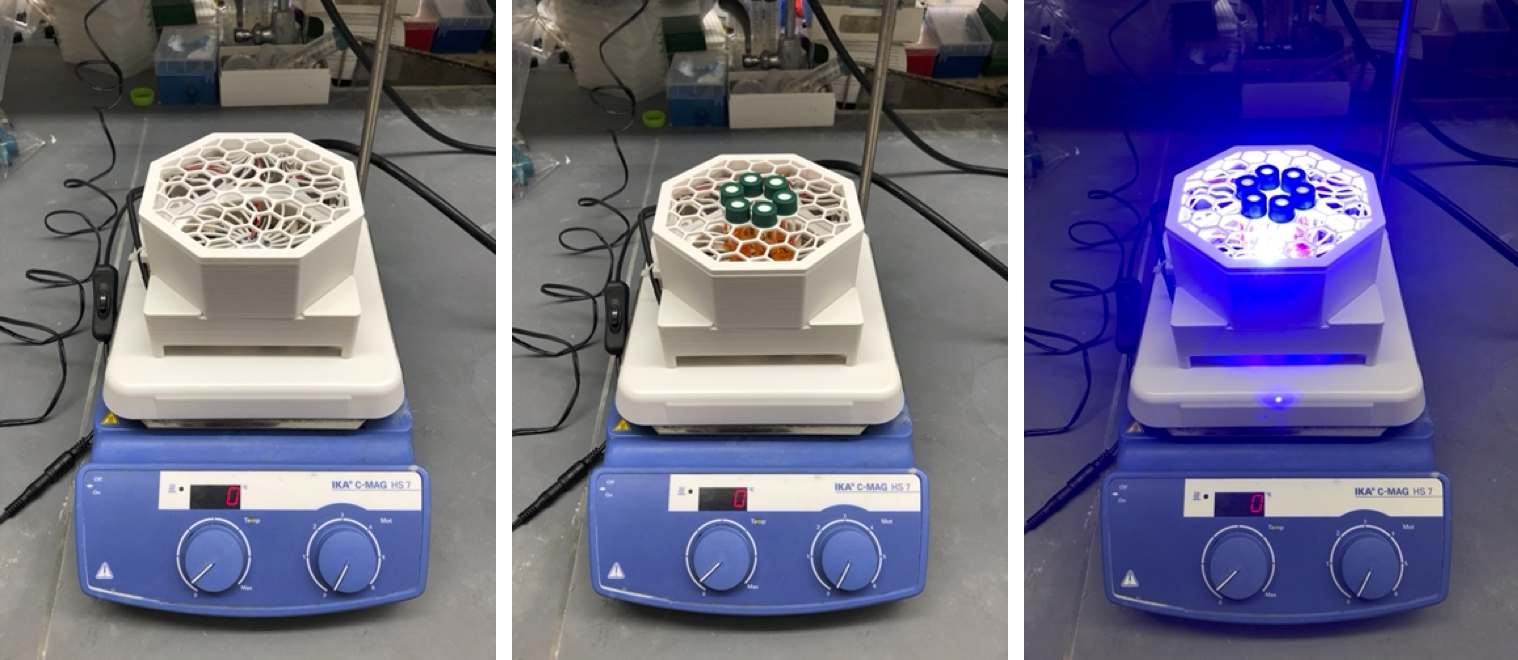
\includegraphics[width=\textwidth]{"./fign8.png"}
  \caption{A WPP apparatus with a 450 nm photon source, 4 mL reactor module and digital driver board on a standard laboratory stir plate conducting 6 simultaneous photoreactions in the multiple reaction configuration.}
\end{figure}

To conduct a photoreaction using a WPP device, an assembled apparatus should be placed on a lab stir plate, to provide reaction mixture stirring, and reaction vessels should be inserted into the apparatus in the desired layout (Figure 23).
The 130 by 130 mm footprint of the WPP architecture is compatible with typical stir plates.
A standard 12 V power supply can then be plugged into the reactor driver to turn on the device and start irradiation.
A single 12V 2 A power supply is sufficient to drive 2 WPP devices simultaneously.
A switch can be installed between the WPP apparatus and power supply to provide power switching.

Reaction and photon source cooling is provided by the fan integrated into the base.
Additional cooling can be achieved through placement of fans above the WPP apparatus or by placing a WPP device on a stir plate within a refrigerator or cold room.

Once finished, the WPP apparatus can be switched off by simply unplugging it. The apparatus can be disassembled for storage.

\section{Documentation}

WPP devices are easy to document.
Suggested below are the aspects of a WPP device that one should document whenever a WPP device is used in an investigation. 
Documenting each of these aspects will allow for precise reproduction of the exact WPP device used within a study. 

\subsection{Base and Photon Source} \label{SEC:doc-photon-source}

Users should report the following for each based and photon source used:

\begin{itemize}
	\item Max emission wavelength for LEDs.
	\item Manufacturer and part number for LEDs.
	\item Supplier and part number for LED star (if commercial).
\end{itemize}

This information enables precise reproduction of WPP photon sources. Characterization of a photon source’s emission profile using a spectrometer is recommended but not required for reproduction. Emission profiles for commercial LEDs are supplied in part datasheets provided by manufacturers.

\subsection{Reaction Module} \label{SEC:doc-reaction modules}

Users should provide and report the following for each reaction module used:

\begin{itemize}
	\item Original CAD designs for both module parts.
	\item 3D-printable models for both module parts.
	\item Photos of each reaction vessel placement configuration.
	\item Manufacturer and part number for reaction vessel.
\end{itemize}

These provisions enable precise reproduction of reaction modules. Documenting the height a vessel is held above the photon source is recommended but not required for reaction module reproduction. All reaction modules provided in the project repository hold vessels a standardized 7 mm above the photon source.

\subsection{Reactor Driver Electronics} \label{SEC:doc-reactor-drivers}

As each reactor driver offers different configurational abilities, each requires different levels of documentation for exact reproduction.

\subsubsection{Analog Driver Board } \label{SEC:doc-analog-driver}

Users should report the following when an analog driver board is used:

\begin{itemize}
	\item Measured test point voltage.
	\item Relative intensity at which LEDs are driven (0 to 100\%).
\end{itemize}

These provisions enable precise reproduction of reaction conditions for transformations carried out using WPP devices fitted with analog driver boards.

\subsubsection{Digital Driver Board} \label{SEC:doc-digital-driver}

Users should provide and document the following when a digital driver board is used:

\begin{itemize}
	\item Firmware used to operate the digital driver board, control unit and any other peripherals.
	\item Relative intensity at which LEDs are driven (0 to 100\%).
	\item Relative fan speed (0 to 100\%).
\end{itemize}

These provisions enable precise reproduction of reaction conditions for transformations carried out using WPP devices fitted with digital driver boards.

\subsubsection{Simple Driver Circuit} \label{SEC:doc-simple-driver}

Users should report the following when a simple LED driver circuit is used:

\begin{itemize}
	\item Manufacturer and part number for LED driver.
\end{itemize}

This information enables reproduction WPP devices fitted with the simple LED driver circuit.

\section{Safety}

WPP reactors utilize high-intensity light emitting diodes (LED) that can cause eye damage if proper safety precautions are not observed.

A light-blocking shield should be utilized whenever operating a WPP apparatus. 
Care must be taken to ensure the light-blocking shield employed adequately blocks light emitted by a WPP photon source from directly reaching a user.

\begin{figure}[H]
	\centering
	\includegraphics[width=\textwidth/2]{"./fig24.png"}
	\caption{WPP device fitted the provided light shield cover module printed in black PLA.}
\end{figure}

A 3D printable light-blocking cover module for WPP devices is provided in the 'photoreactor-light-shield' subdirectory of the project repository.
The WPP light shield prevents direct exposure of users to light emitted by WPP photon sources. 
We recommend printing the WPP light shield using black filament is recommended to reduce light bounce (Figure 24).

Use of light-filtering safety glasses alongside a light-blocking shield can provide additional protection from high-intensity light.

\section{Acknowledgments}

We thank Dr. Ilia A. Guzei and Sebastian Thompson of UW-Madison for photography and help fabricating custom LED stars, respectively. 

\end{document}
